\section{Introduction to R and HPC}
\makesubcontentsslides

\subsection{Batch and Interactive}

\begin{frame}
  \begin{block}{Data analysis is interactive!}
    \pause
    \begin{itemize}[<+-|alert@+>]
    \item Data reduction to knowledge
    \item S (and R) interactive ``answer'' to batch data analysis
    \item Iterative process with same data
      \begin{itemize}
      \item Diagnostics of fit
      \item Quantification of uncertainty
      \item Interpretation of results
      \end{itemize}
    \item Efficient use of expensive people
    \end{itemize}
  \end{block}
  \begin{block}{Supercomputing is batch!}
    \pause
    \begin{itemize}[<+-|alert@+>]
    \item Traditionally data generation
    \item Long time to assimilate generated data
    \item Efficient use of expensive platforms
    \end{itemize}
  \end{block}
\end{frame}

\subsection{Quick Overview of Parallel Hardware}

\begin{frame}
\begin{block}{Three Basic Flavors of Hardware}
    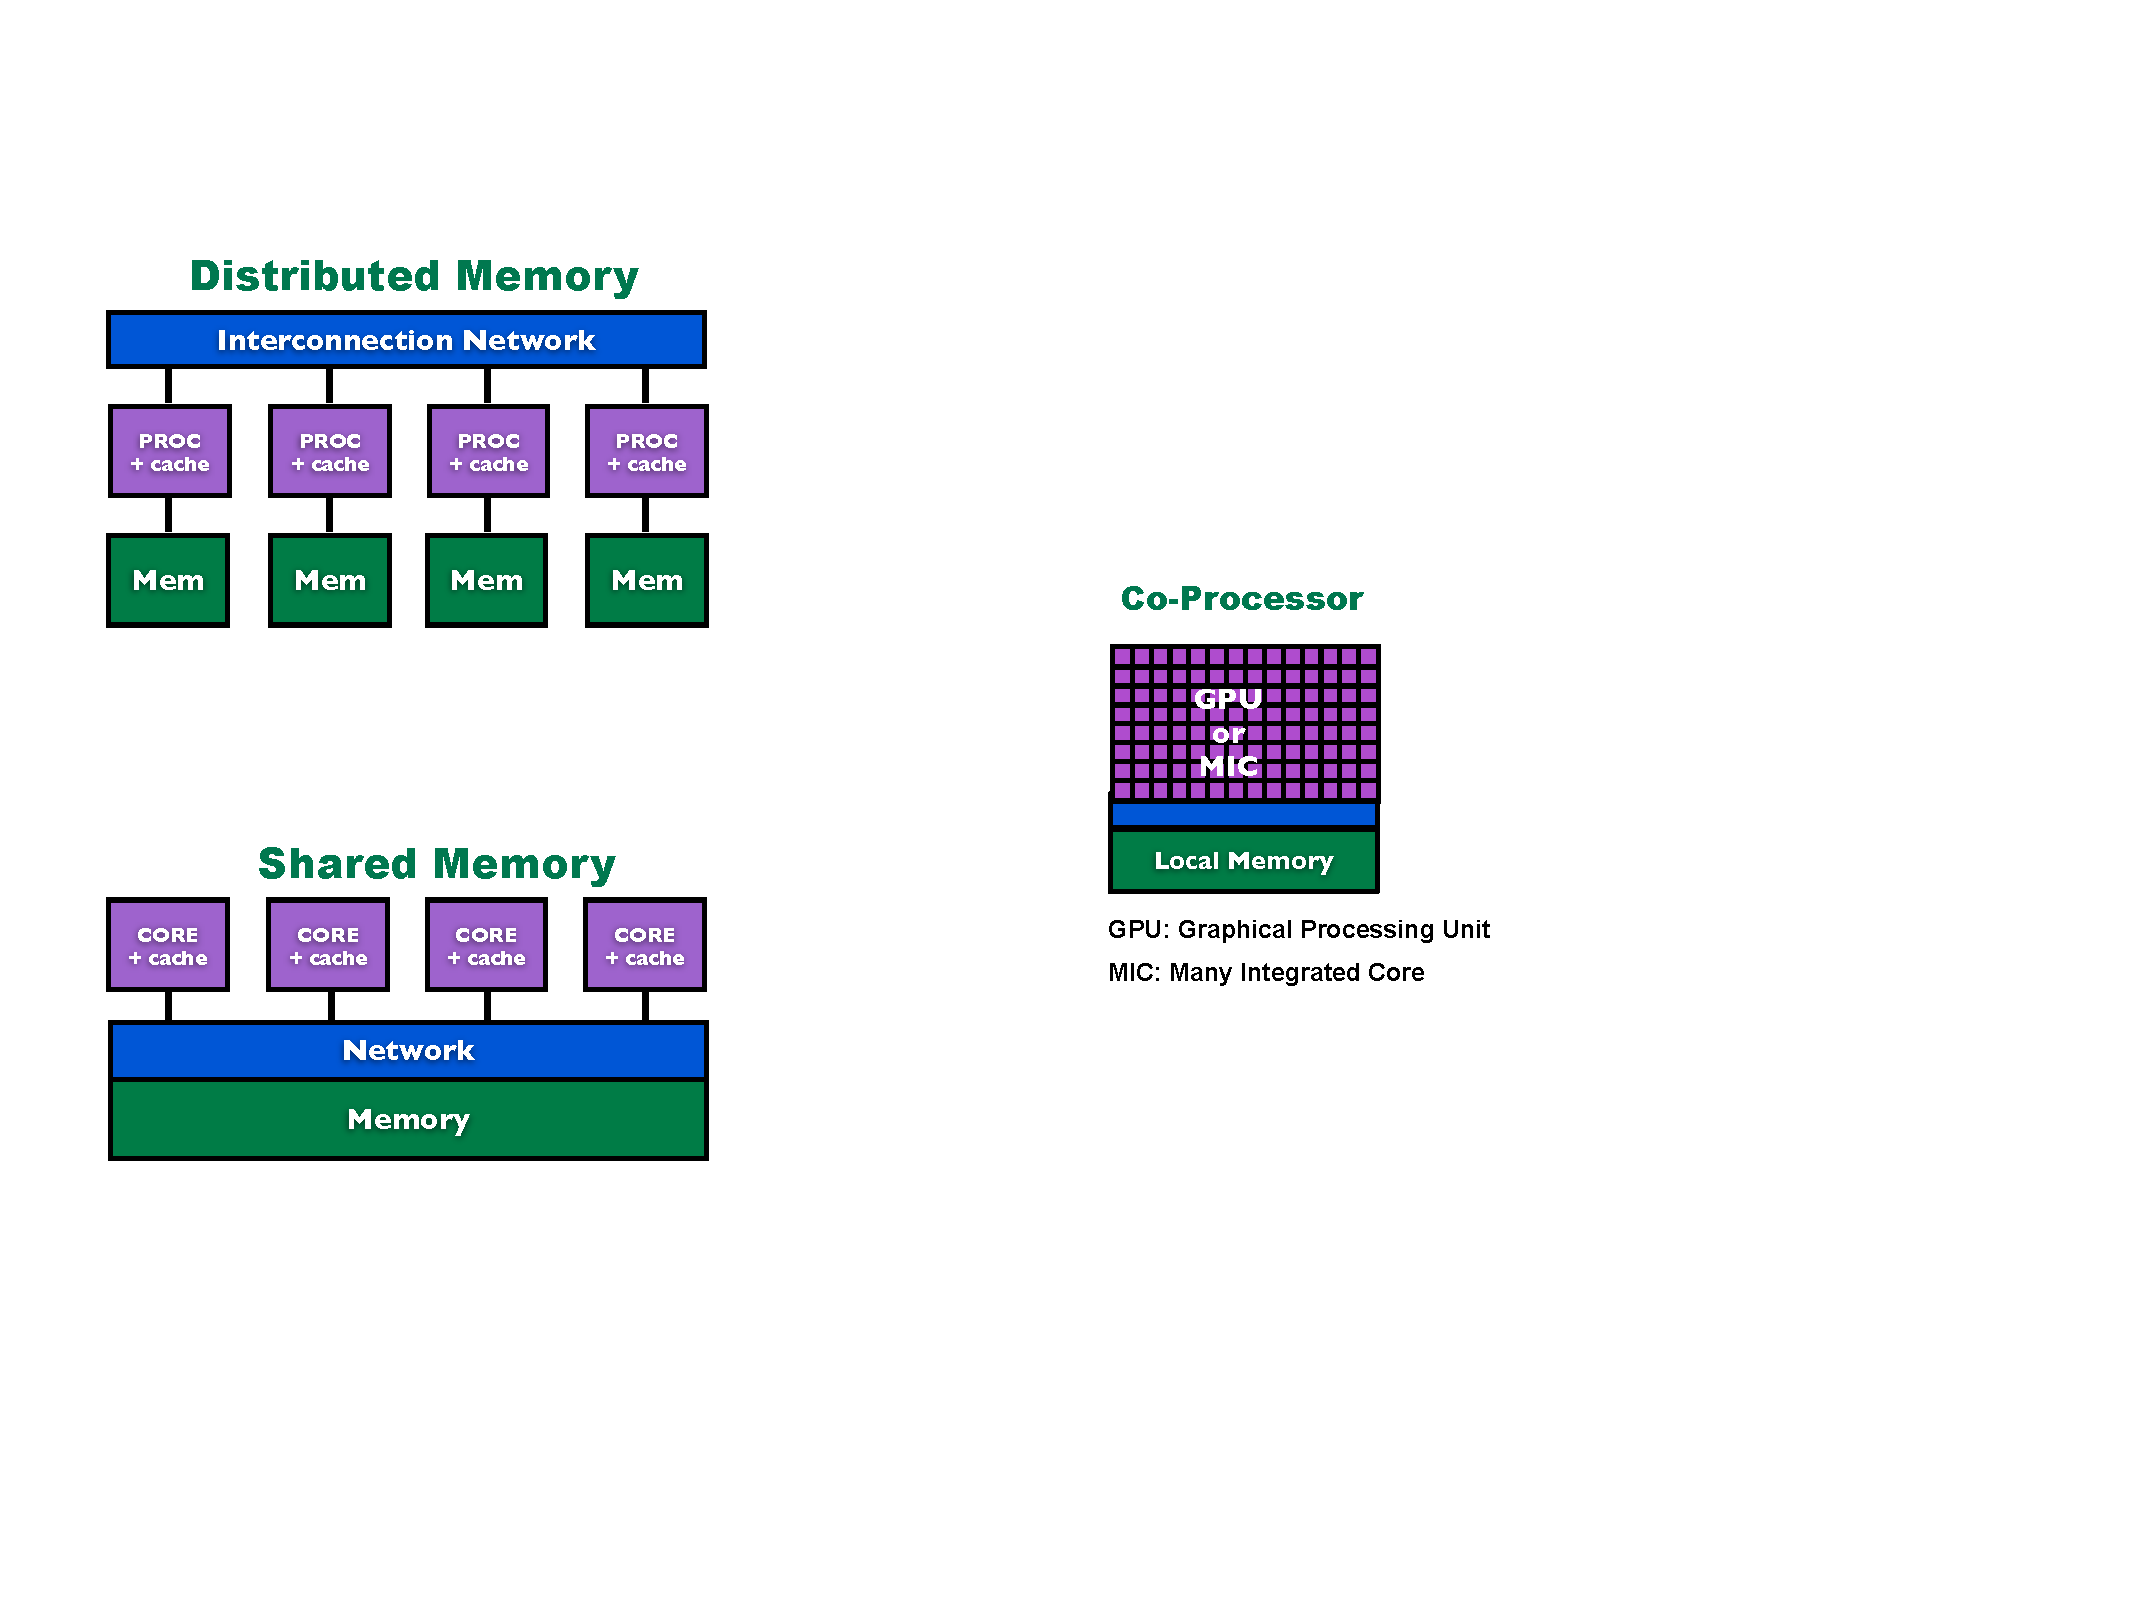
\includegraphics[width=0.95\textwidth]{../common/pics/ParallelHardware1.pdf}
\end{block}
\end{frame}

\begin{frame}
\begin{block}{Your Laptop or Desktop}
    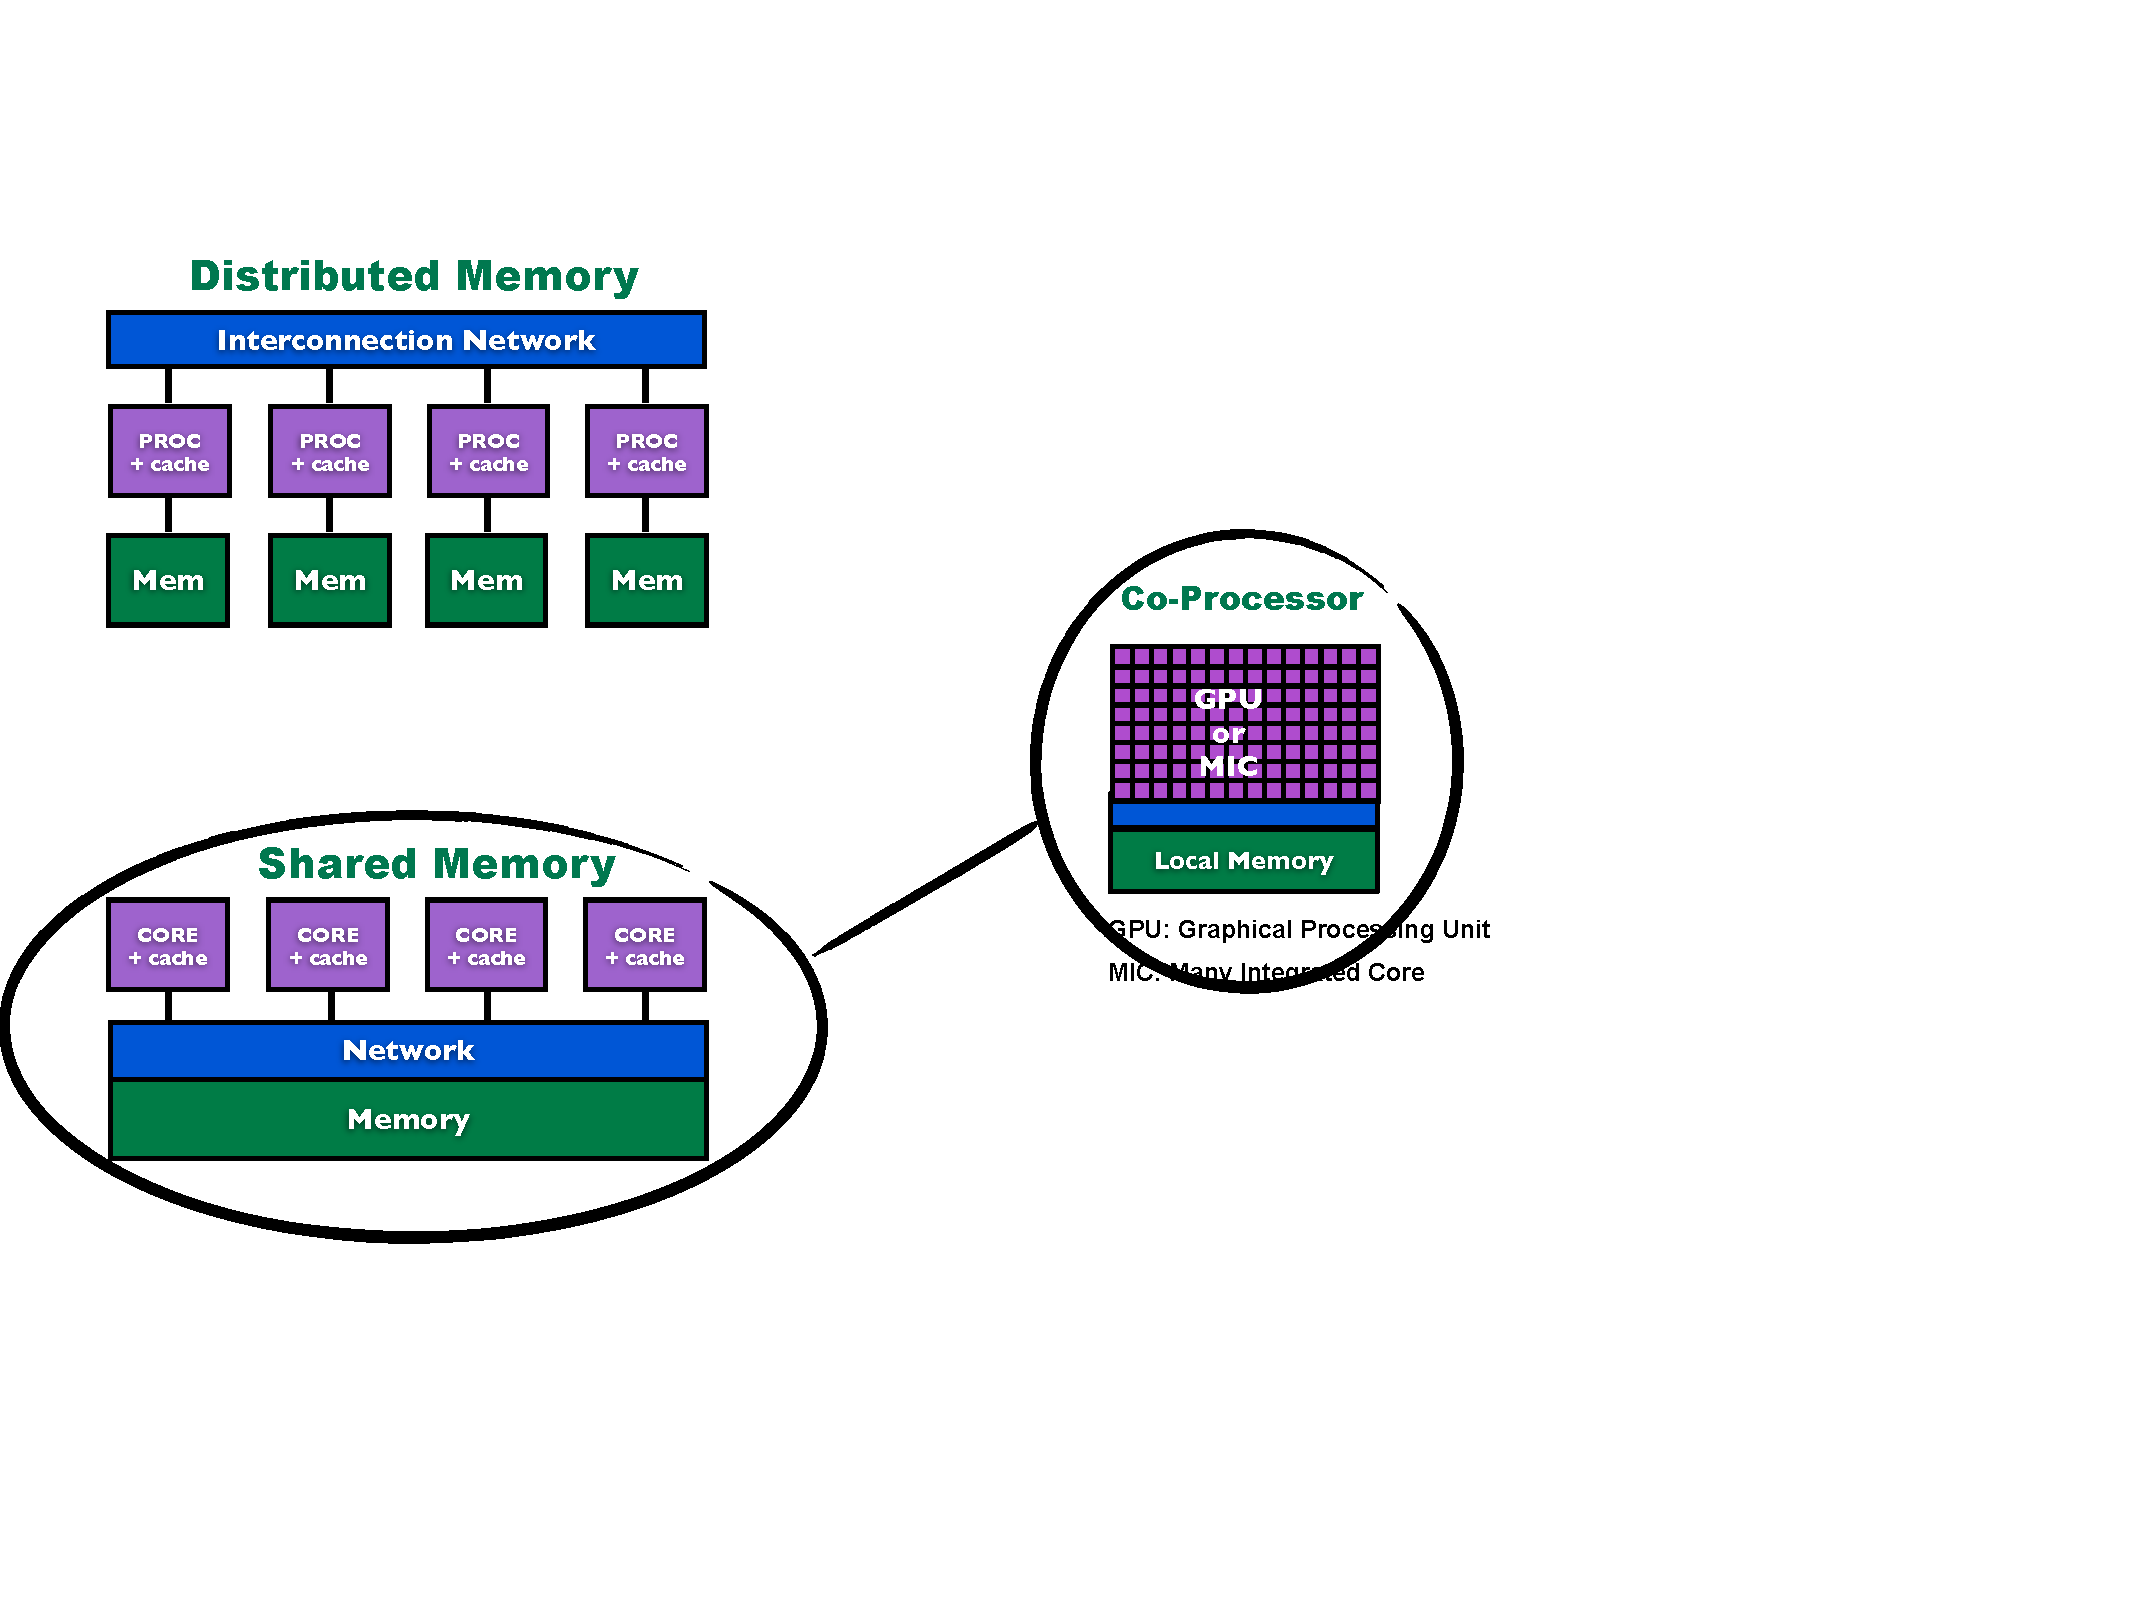
\includegraphics[width=0.95\textwidth]{../common/pics/ParallelHardware2.pdf}
\end{block}
\end{frame}

\begin{frame}
\begin{block}{A Server or Cluster}
    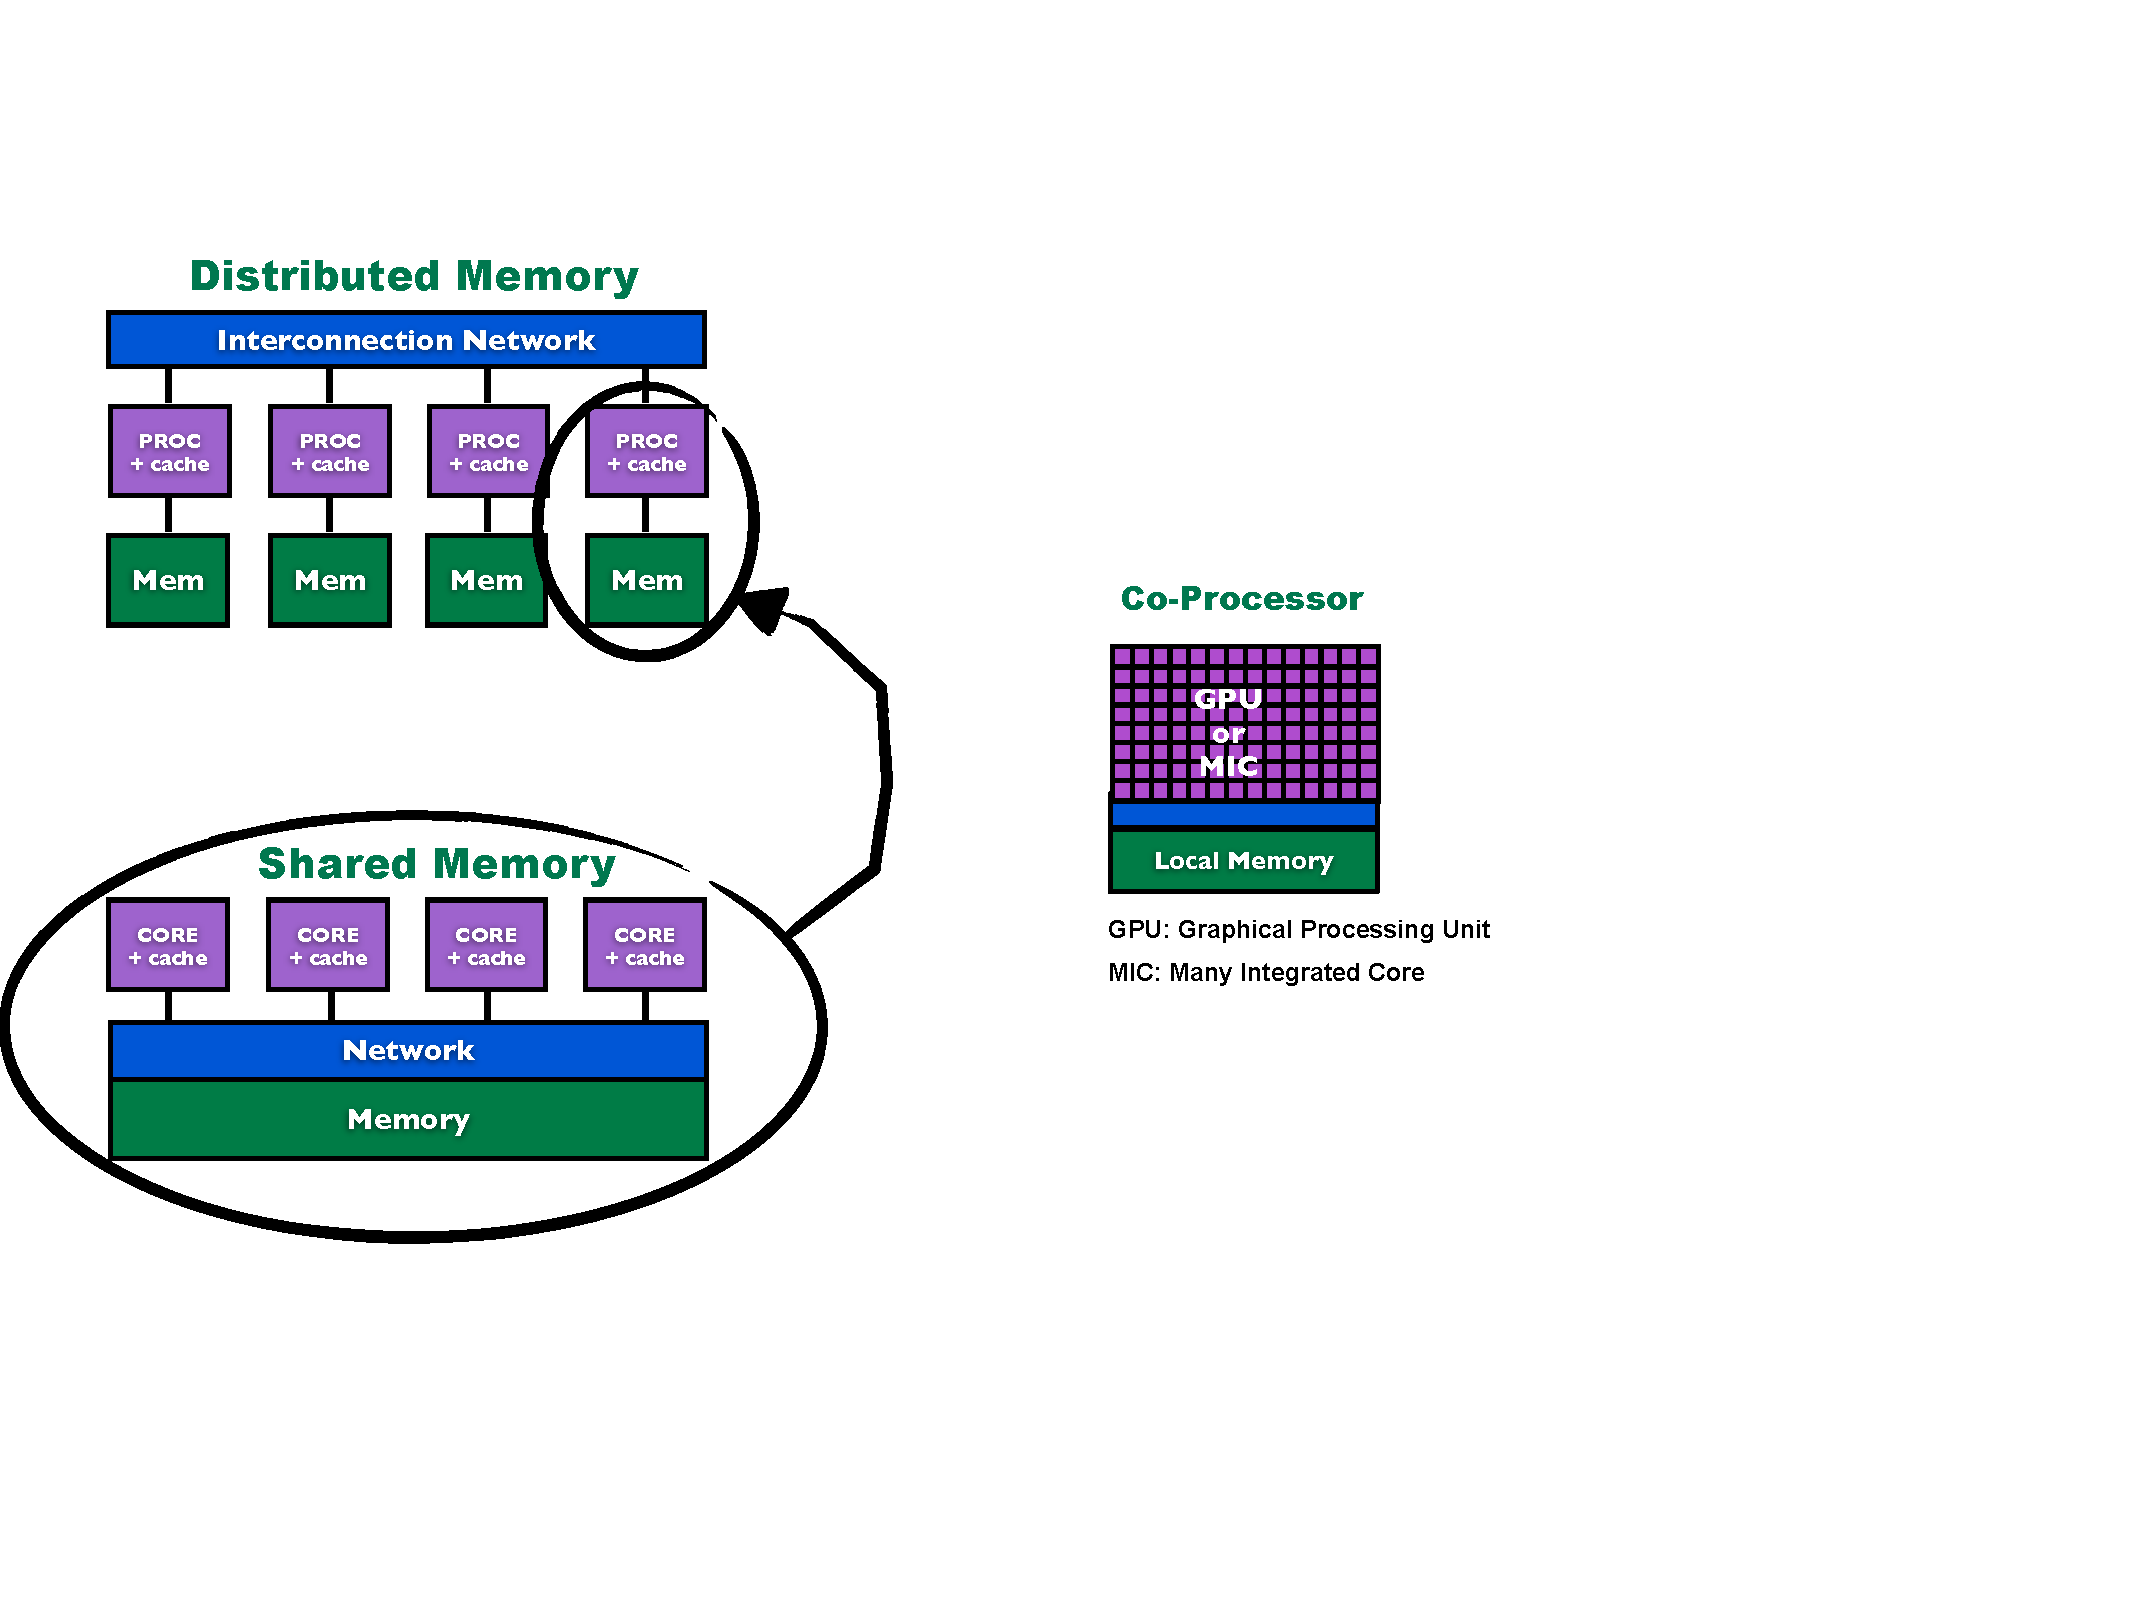
\includegraphics[width=0.95\textwidth]{../common/pics/ParallelHardware3.pdf}
\end{block}
\end{frame}

\begin{frame}
\begin{block}{Server to Supercomputer}
    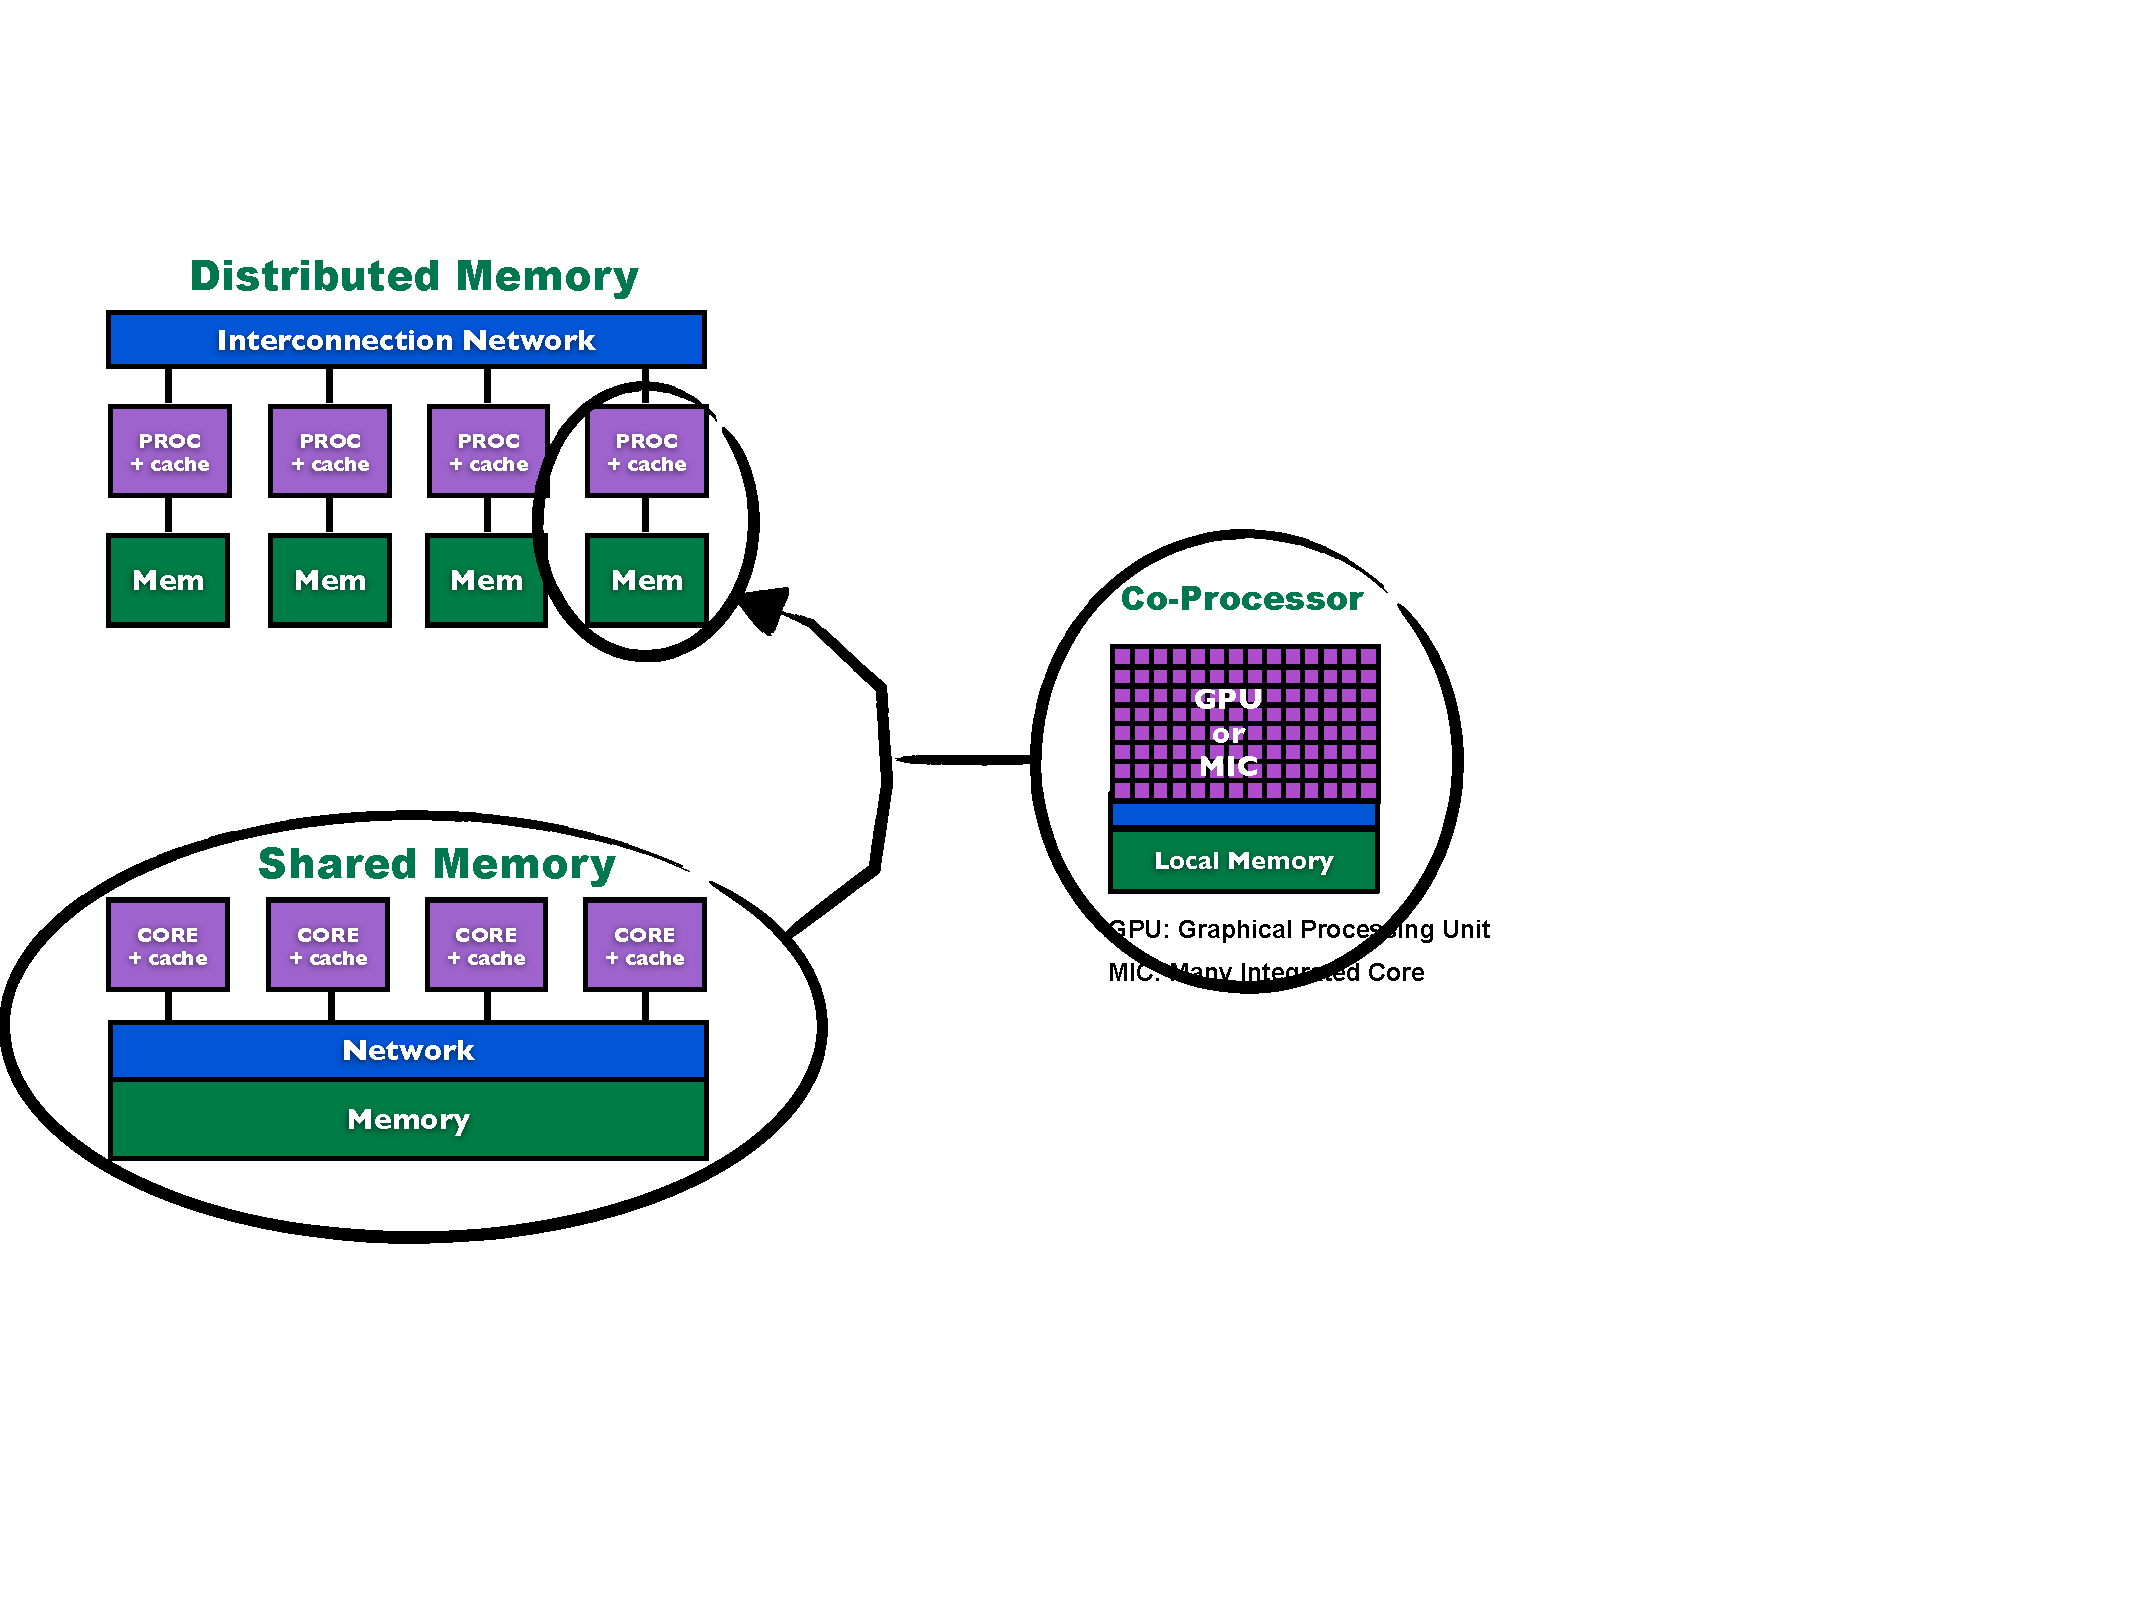
\includegraphics[width=0.95\textwidth]{../common/pics/ParallelHardware4.pdf}
\end{block}
\end{frame}

\begin{frame}
\begin{block}{Knowing the Right Words}
    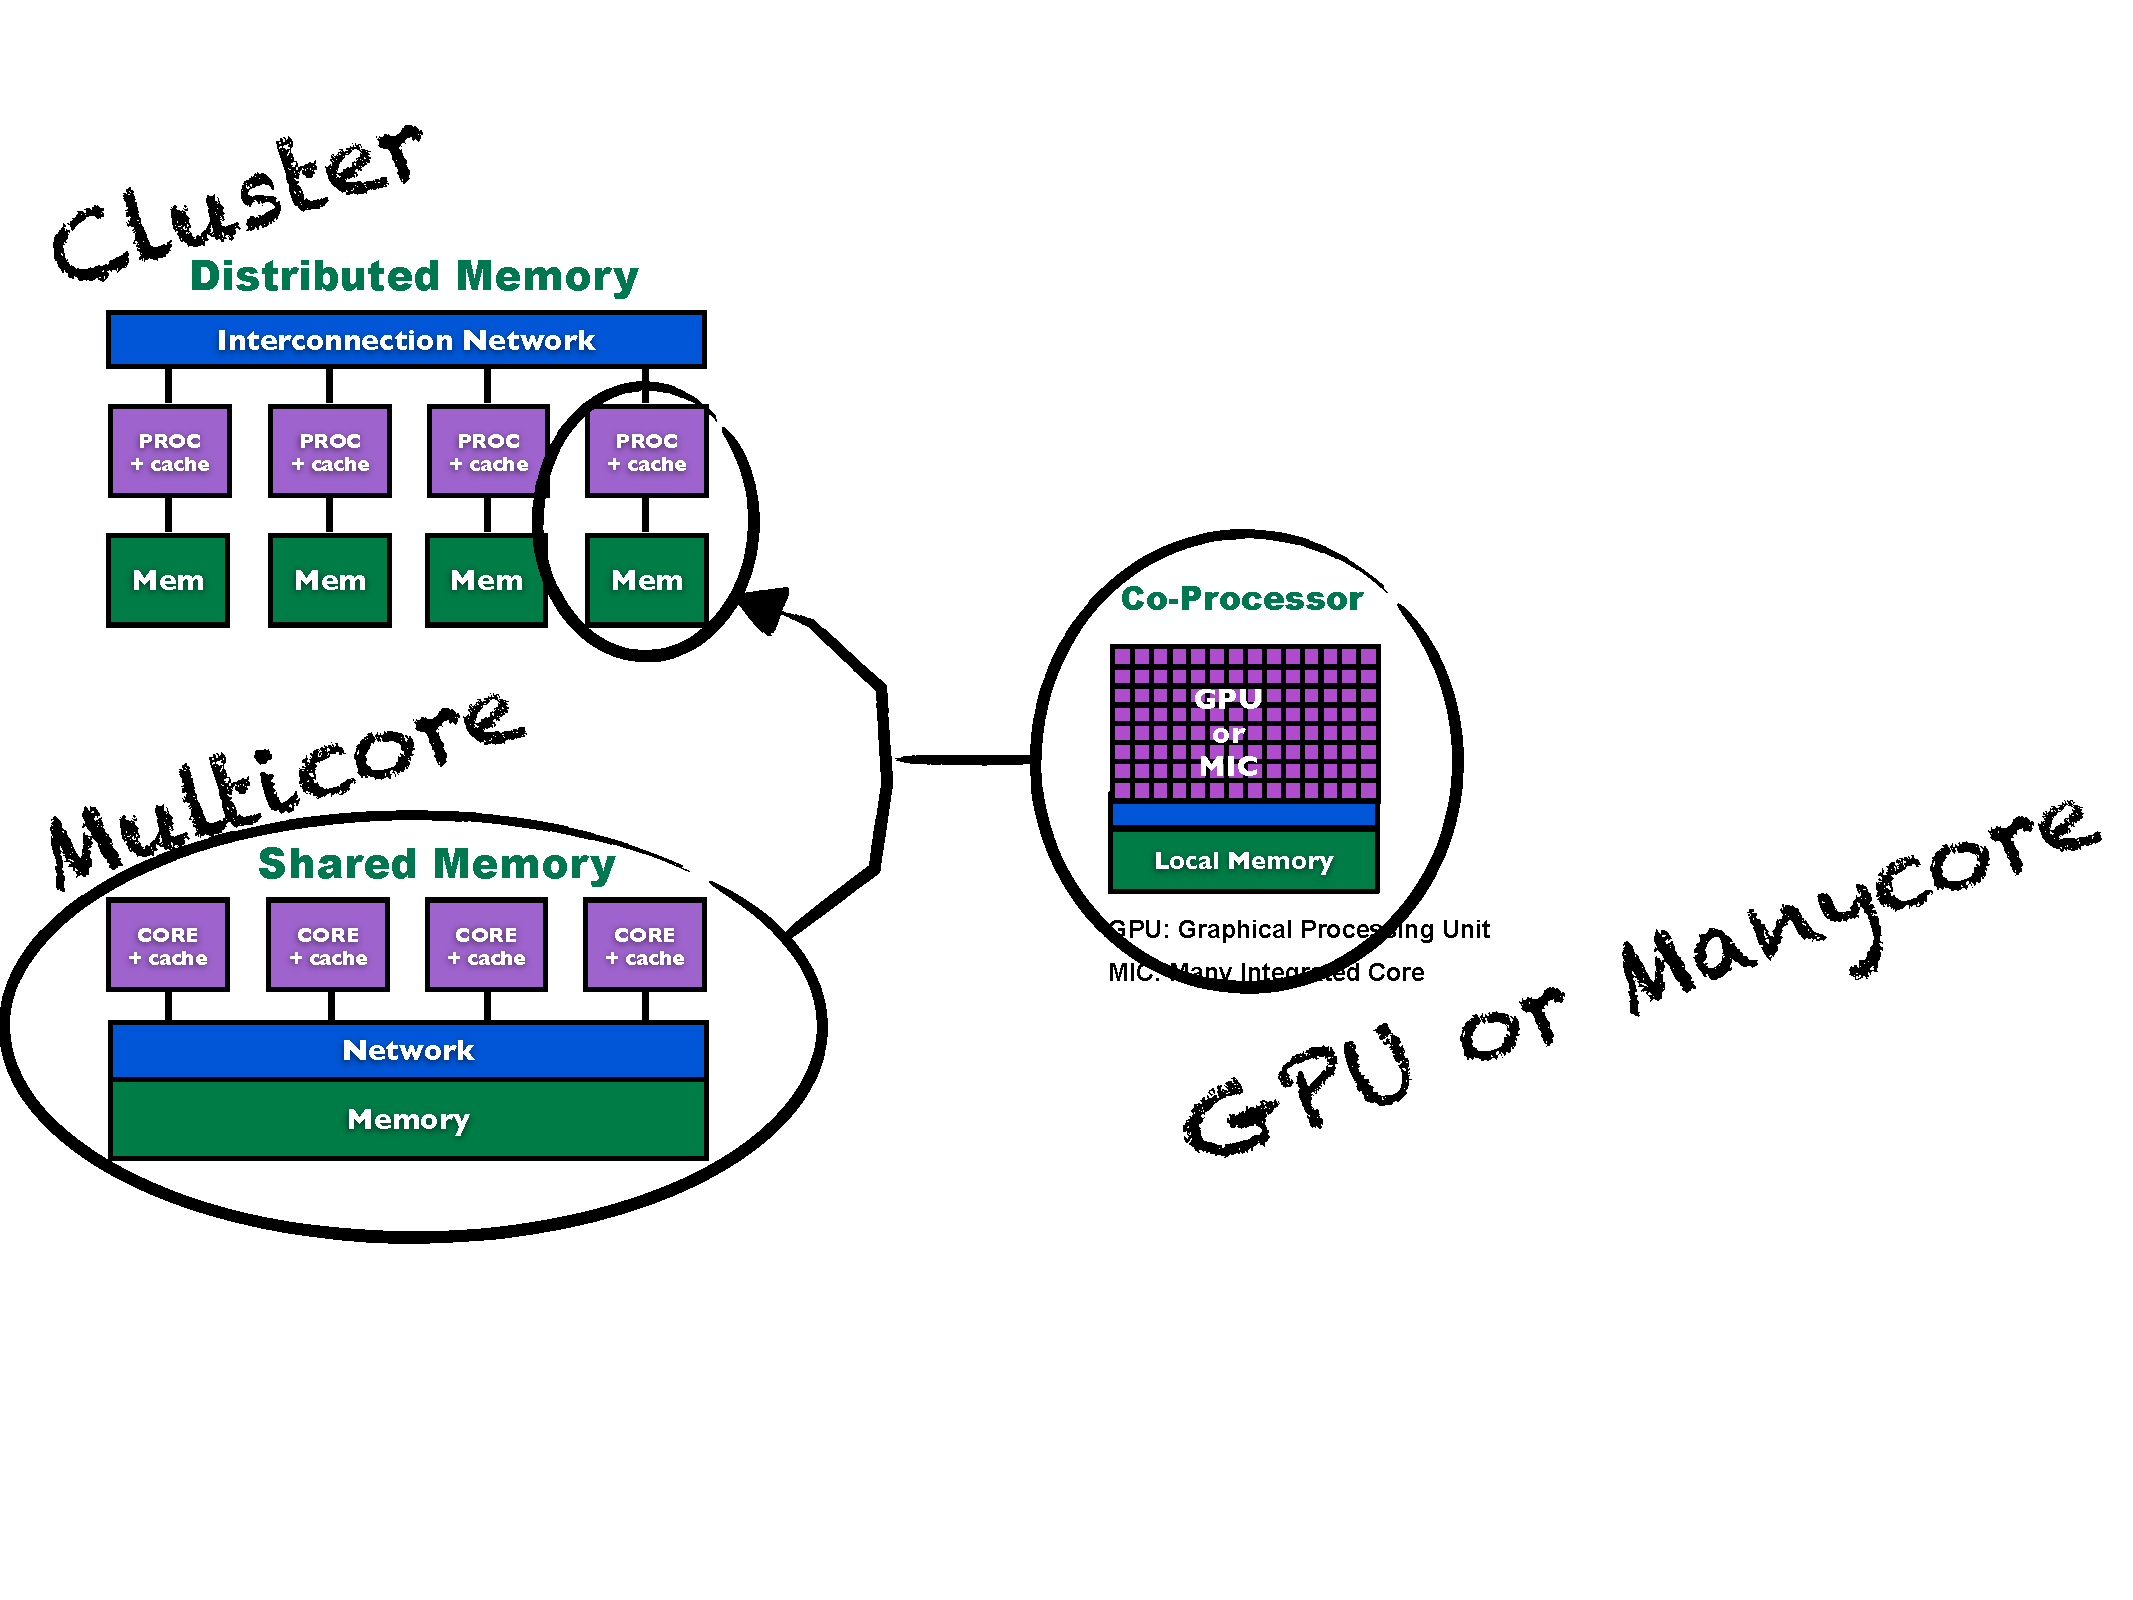
\includegraphics[width=0.95\textwidth]{../common/pics/ParallelHardware5.pdf}
\end{block}
\end{frame}

\begin{frame}
\begin{block}{``Native'' Programming Models and Tools}
    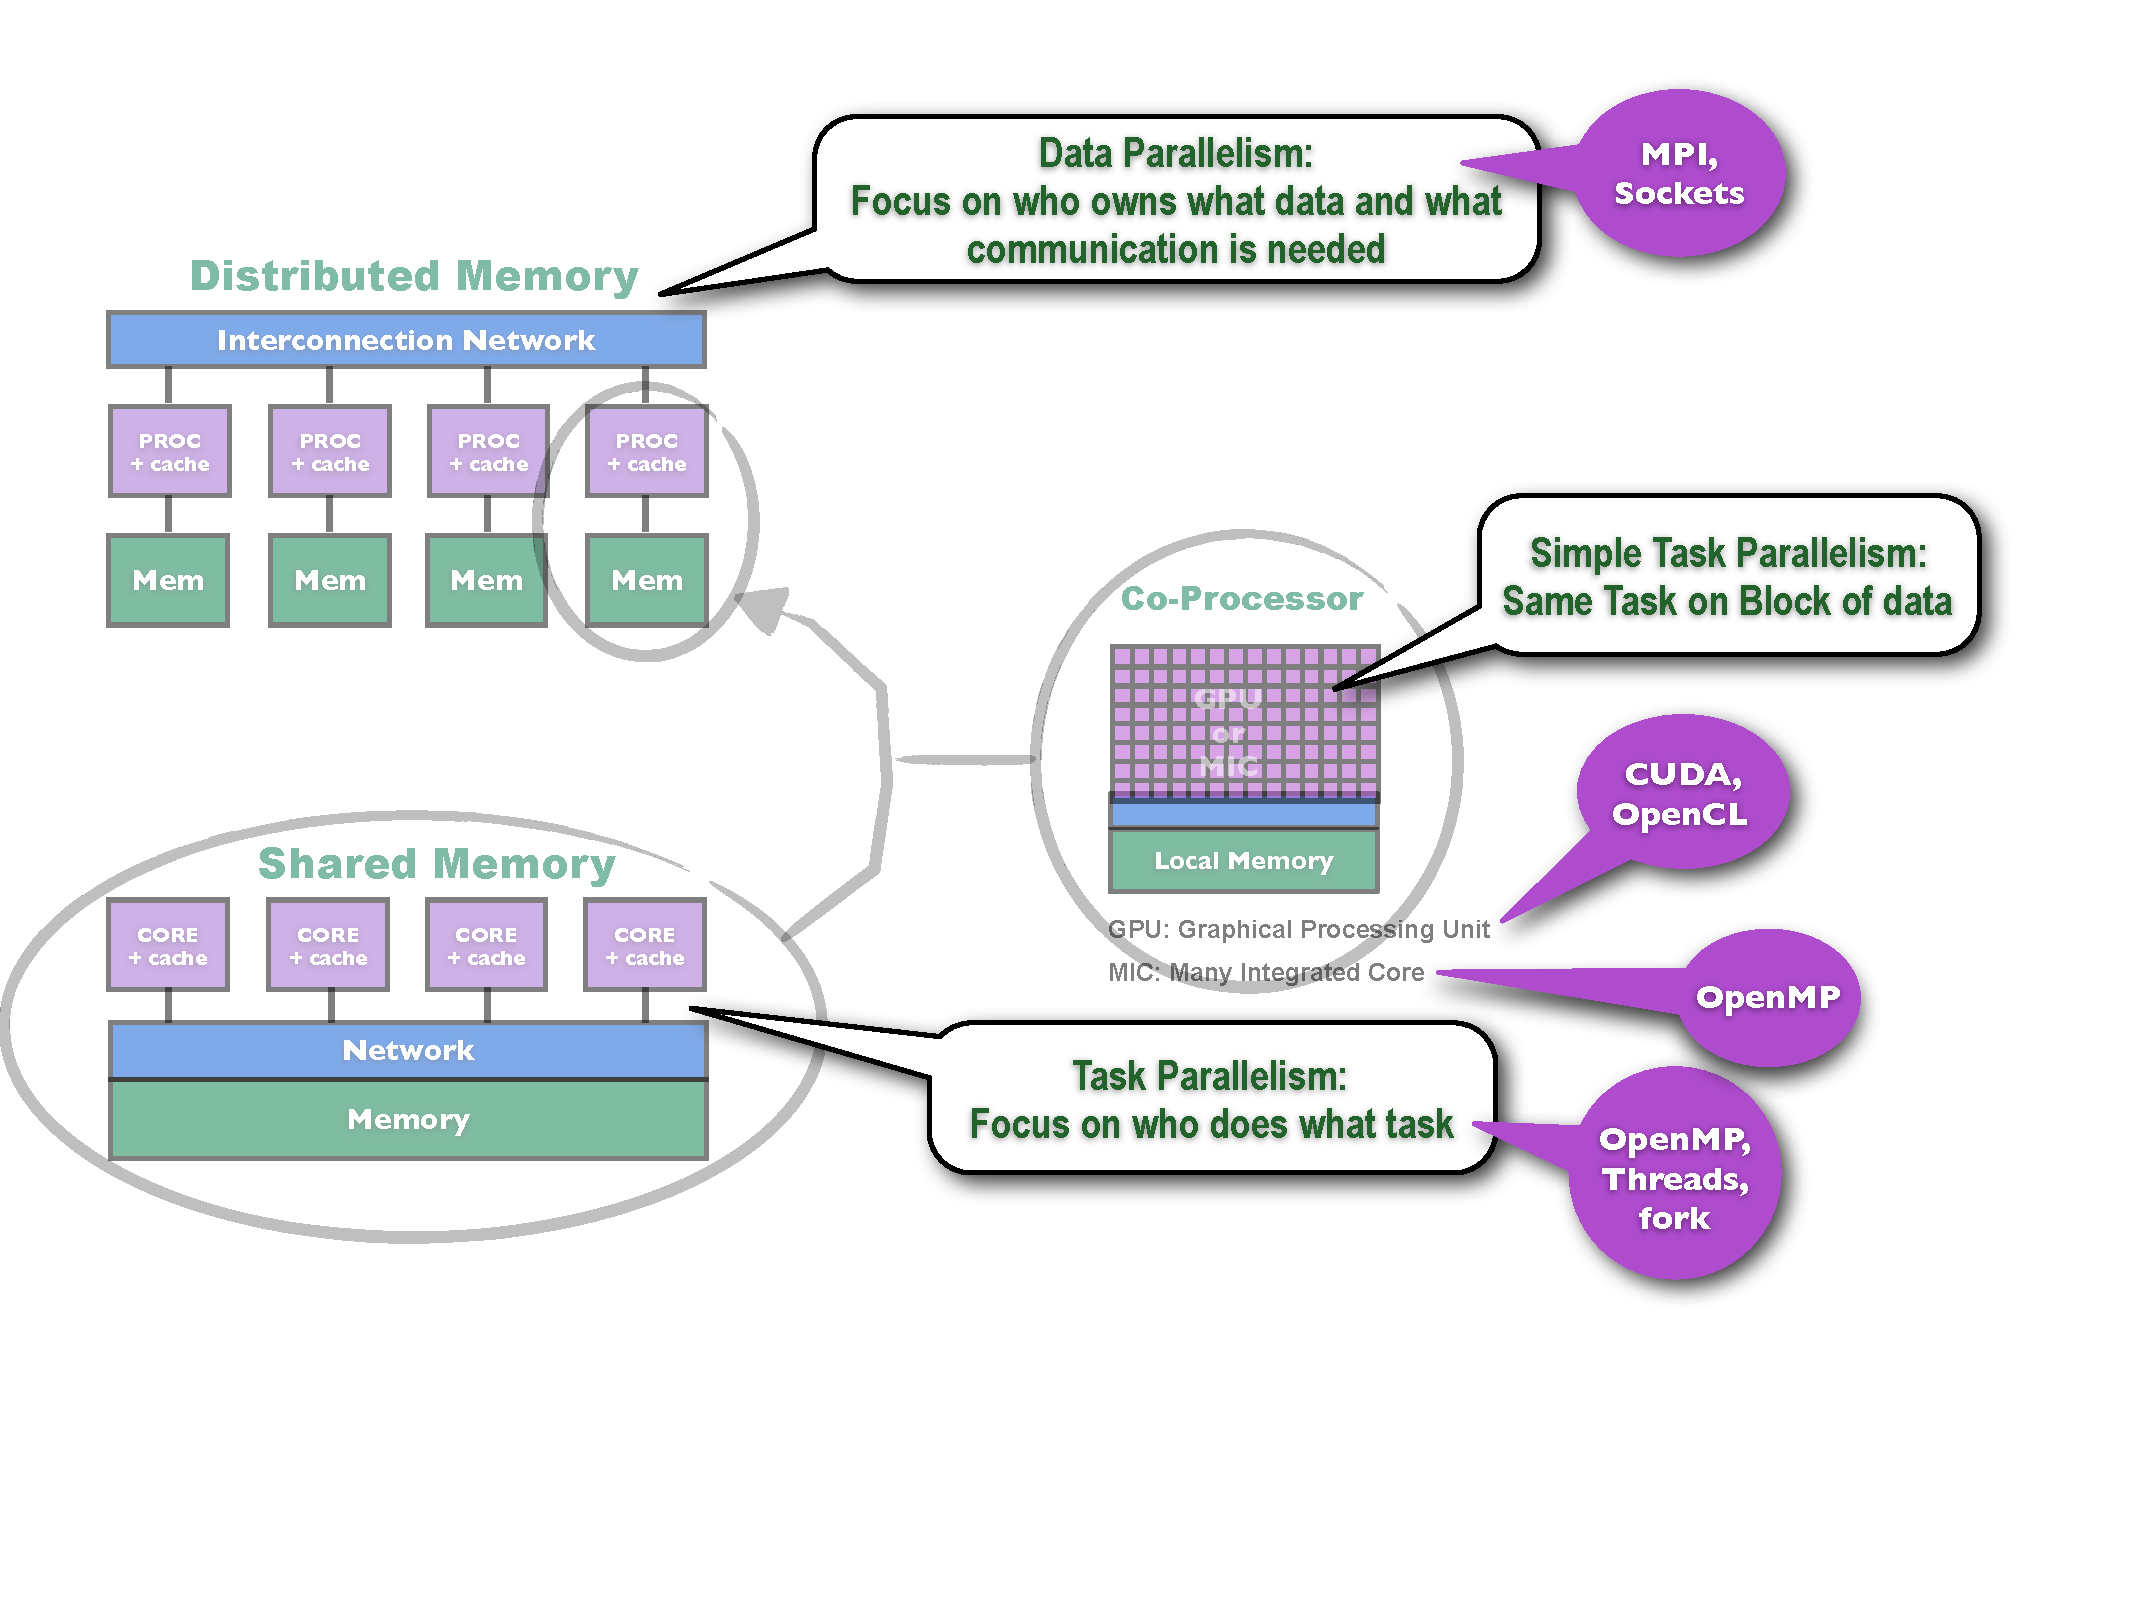
\includegraphics[width=0.95\textwidth]{../common/pics/ParallelHardware6.pdf}
\end{block}
\end{frame}

\begin{frame}
\begin{block}{R Interfaces to Native Tools}
    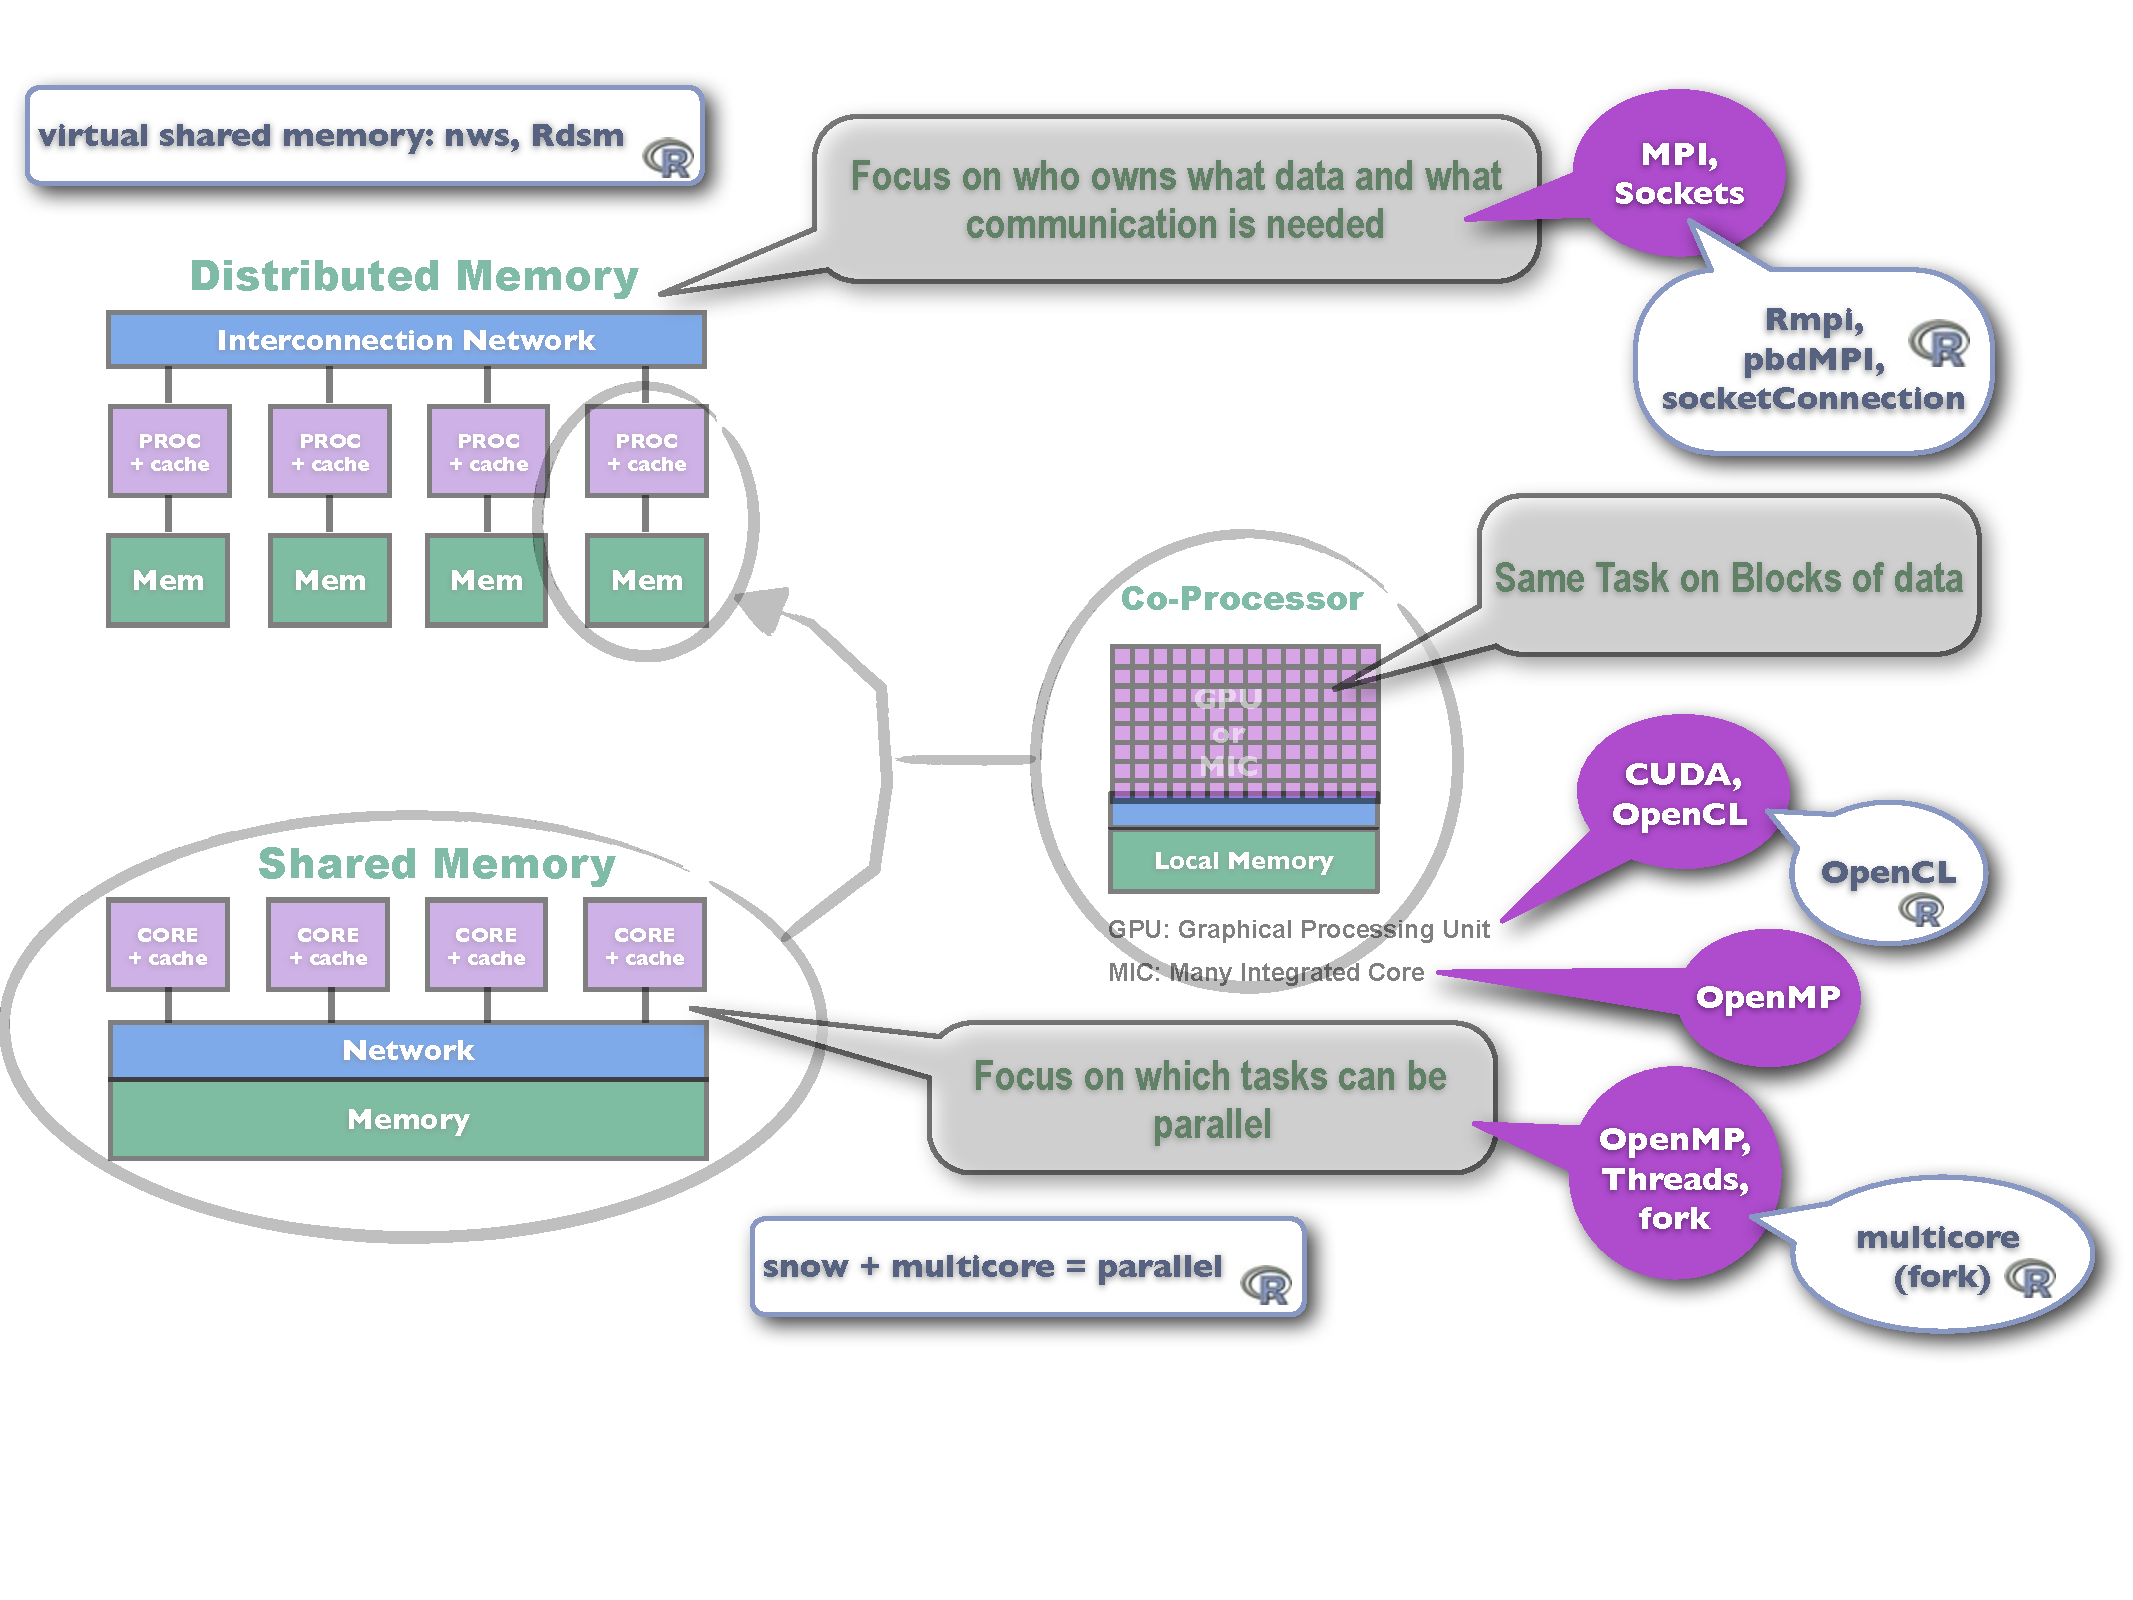
\includegraphics[width=0.95\textwidth]{../common/pics/ParallelHardware7.pdf}
\end{block}
\end{frame}

\begin{frame}
\begin{block}{30+ Years of Parallel Computing Research}
    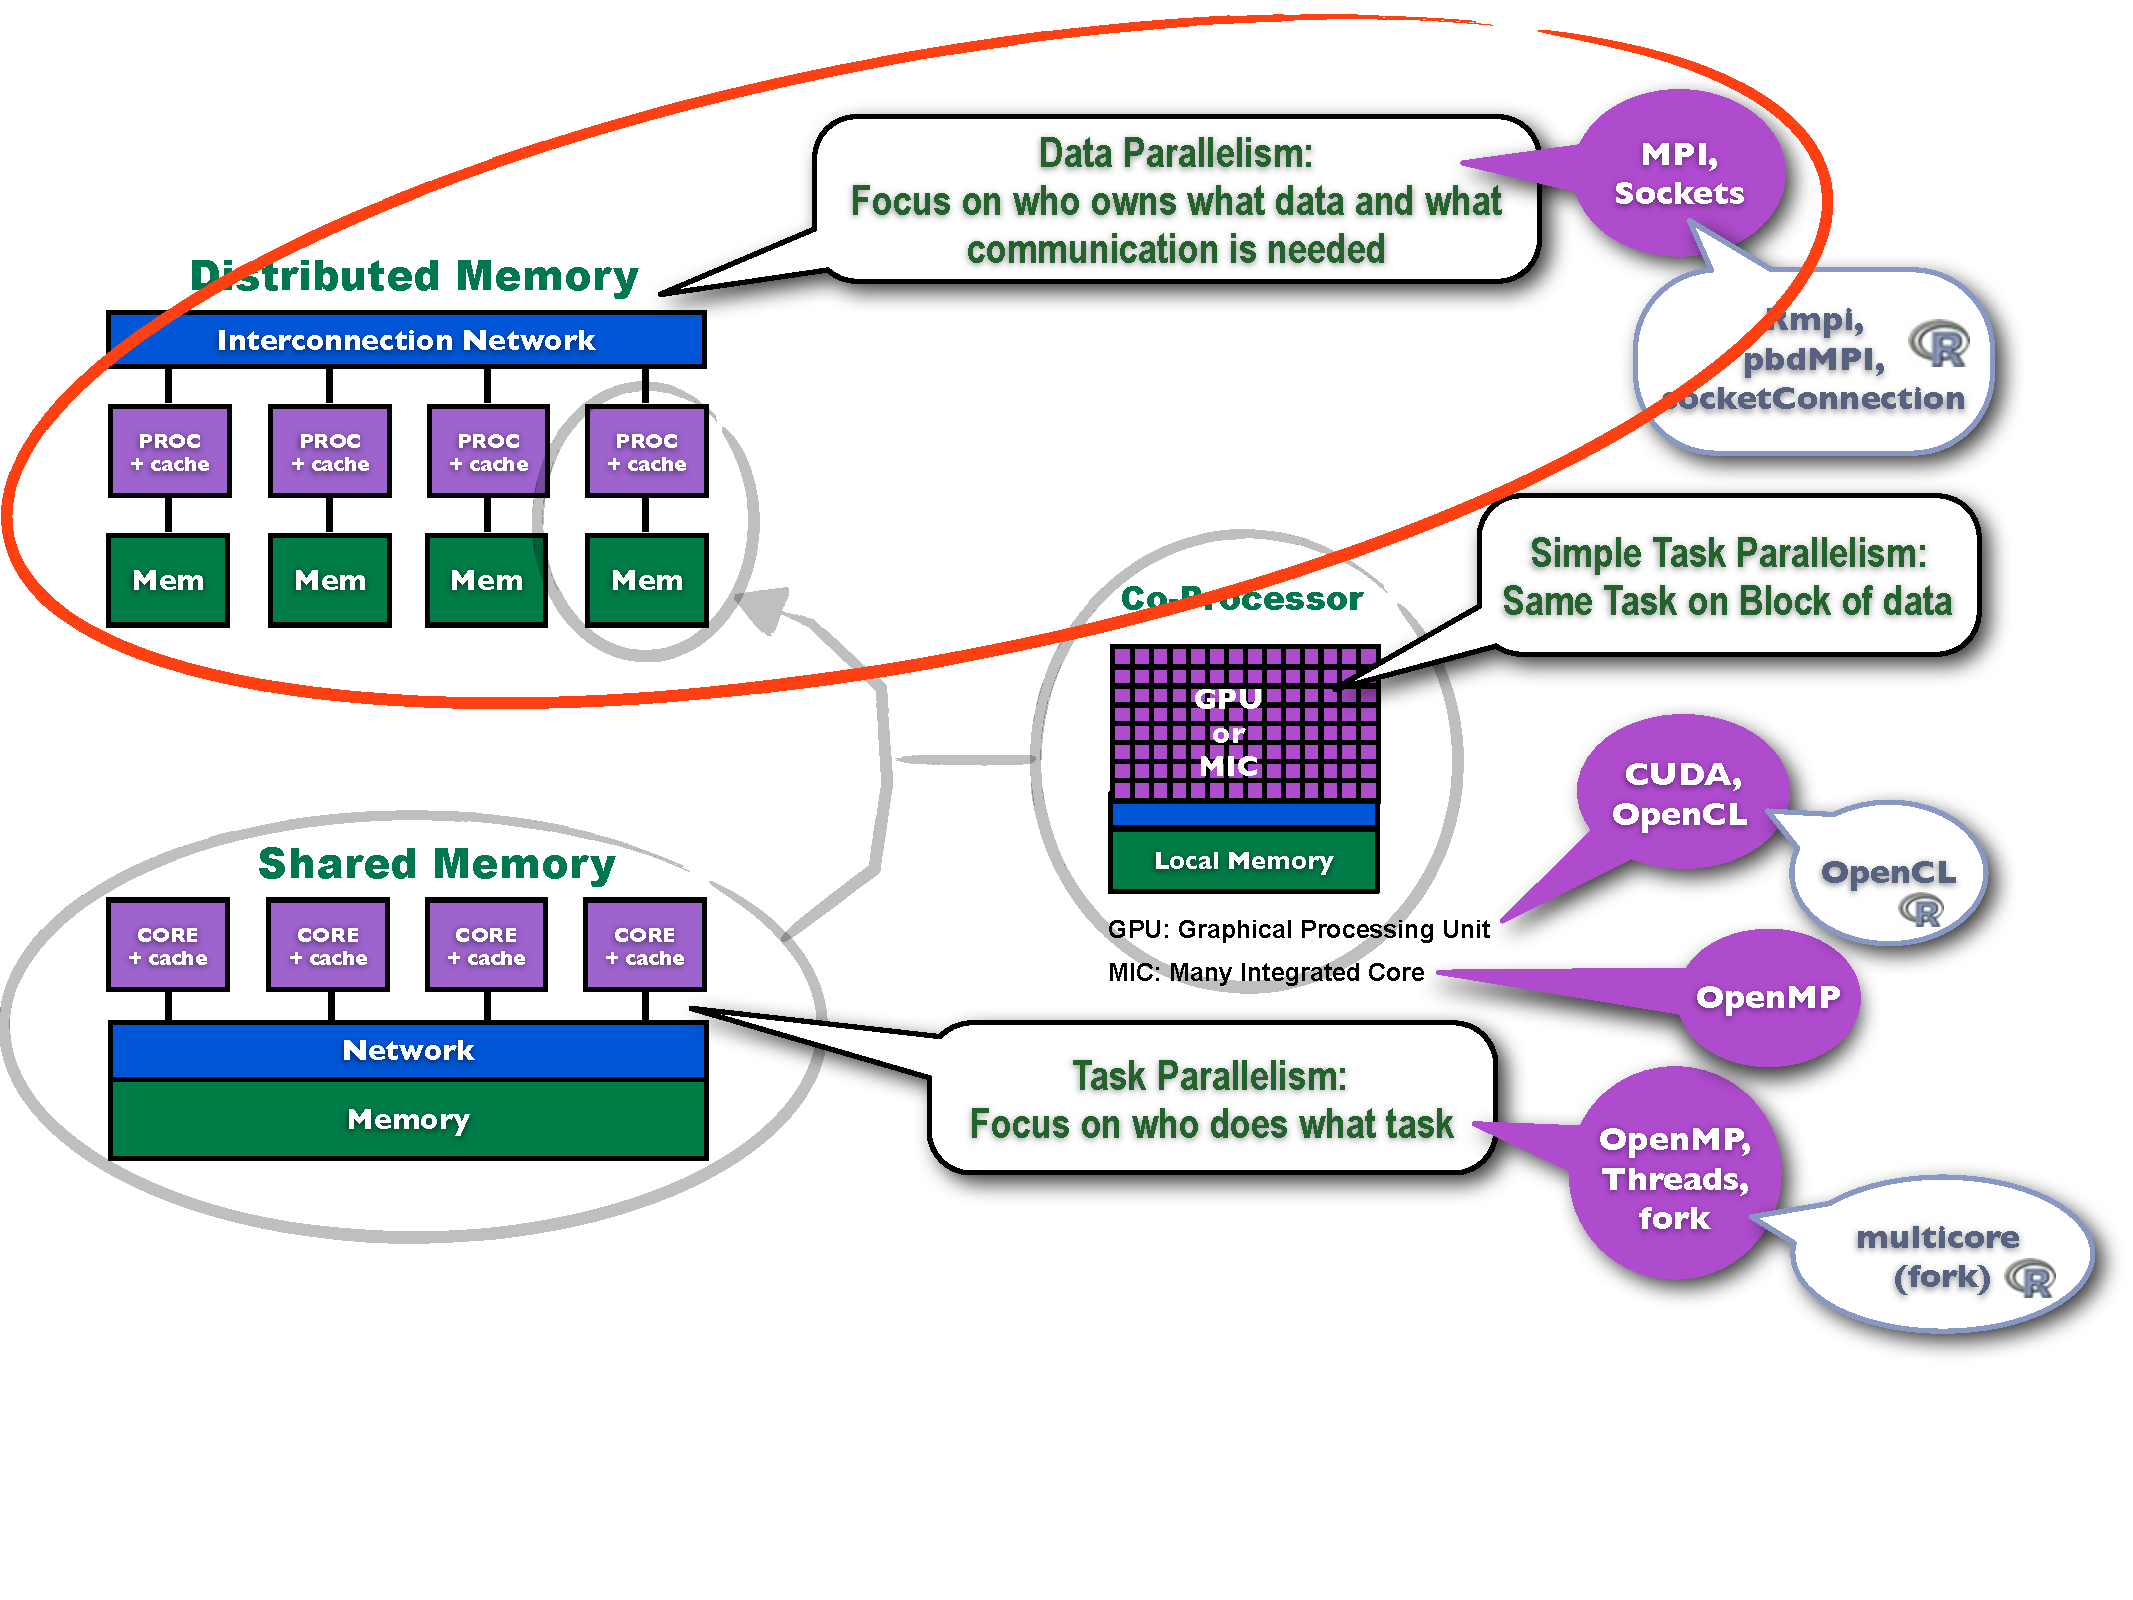
\includegraphics[width=0.95\textwidth]{../common/pics/ParallelHardware8.pdf}
\end{block}
\end{frame}

\begin{frame}
\begin{block}{Last 10 years of Advances}
    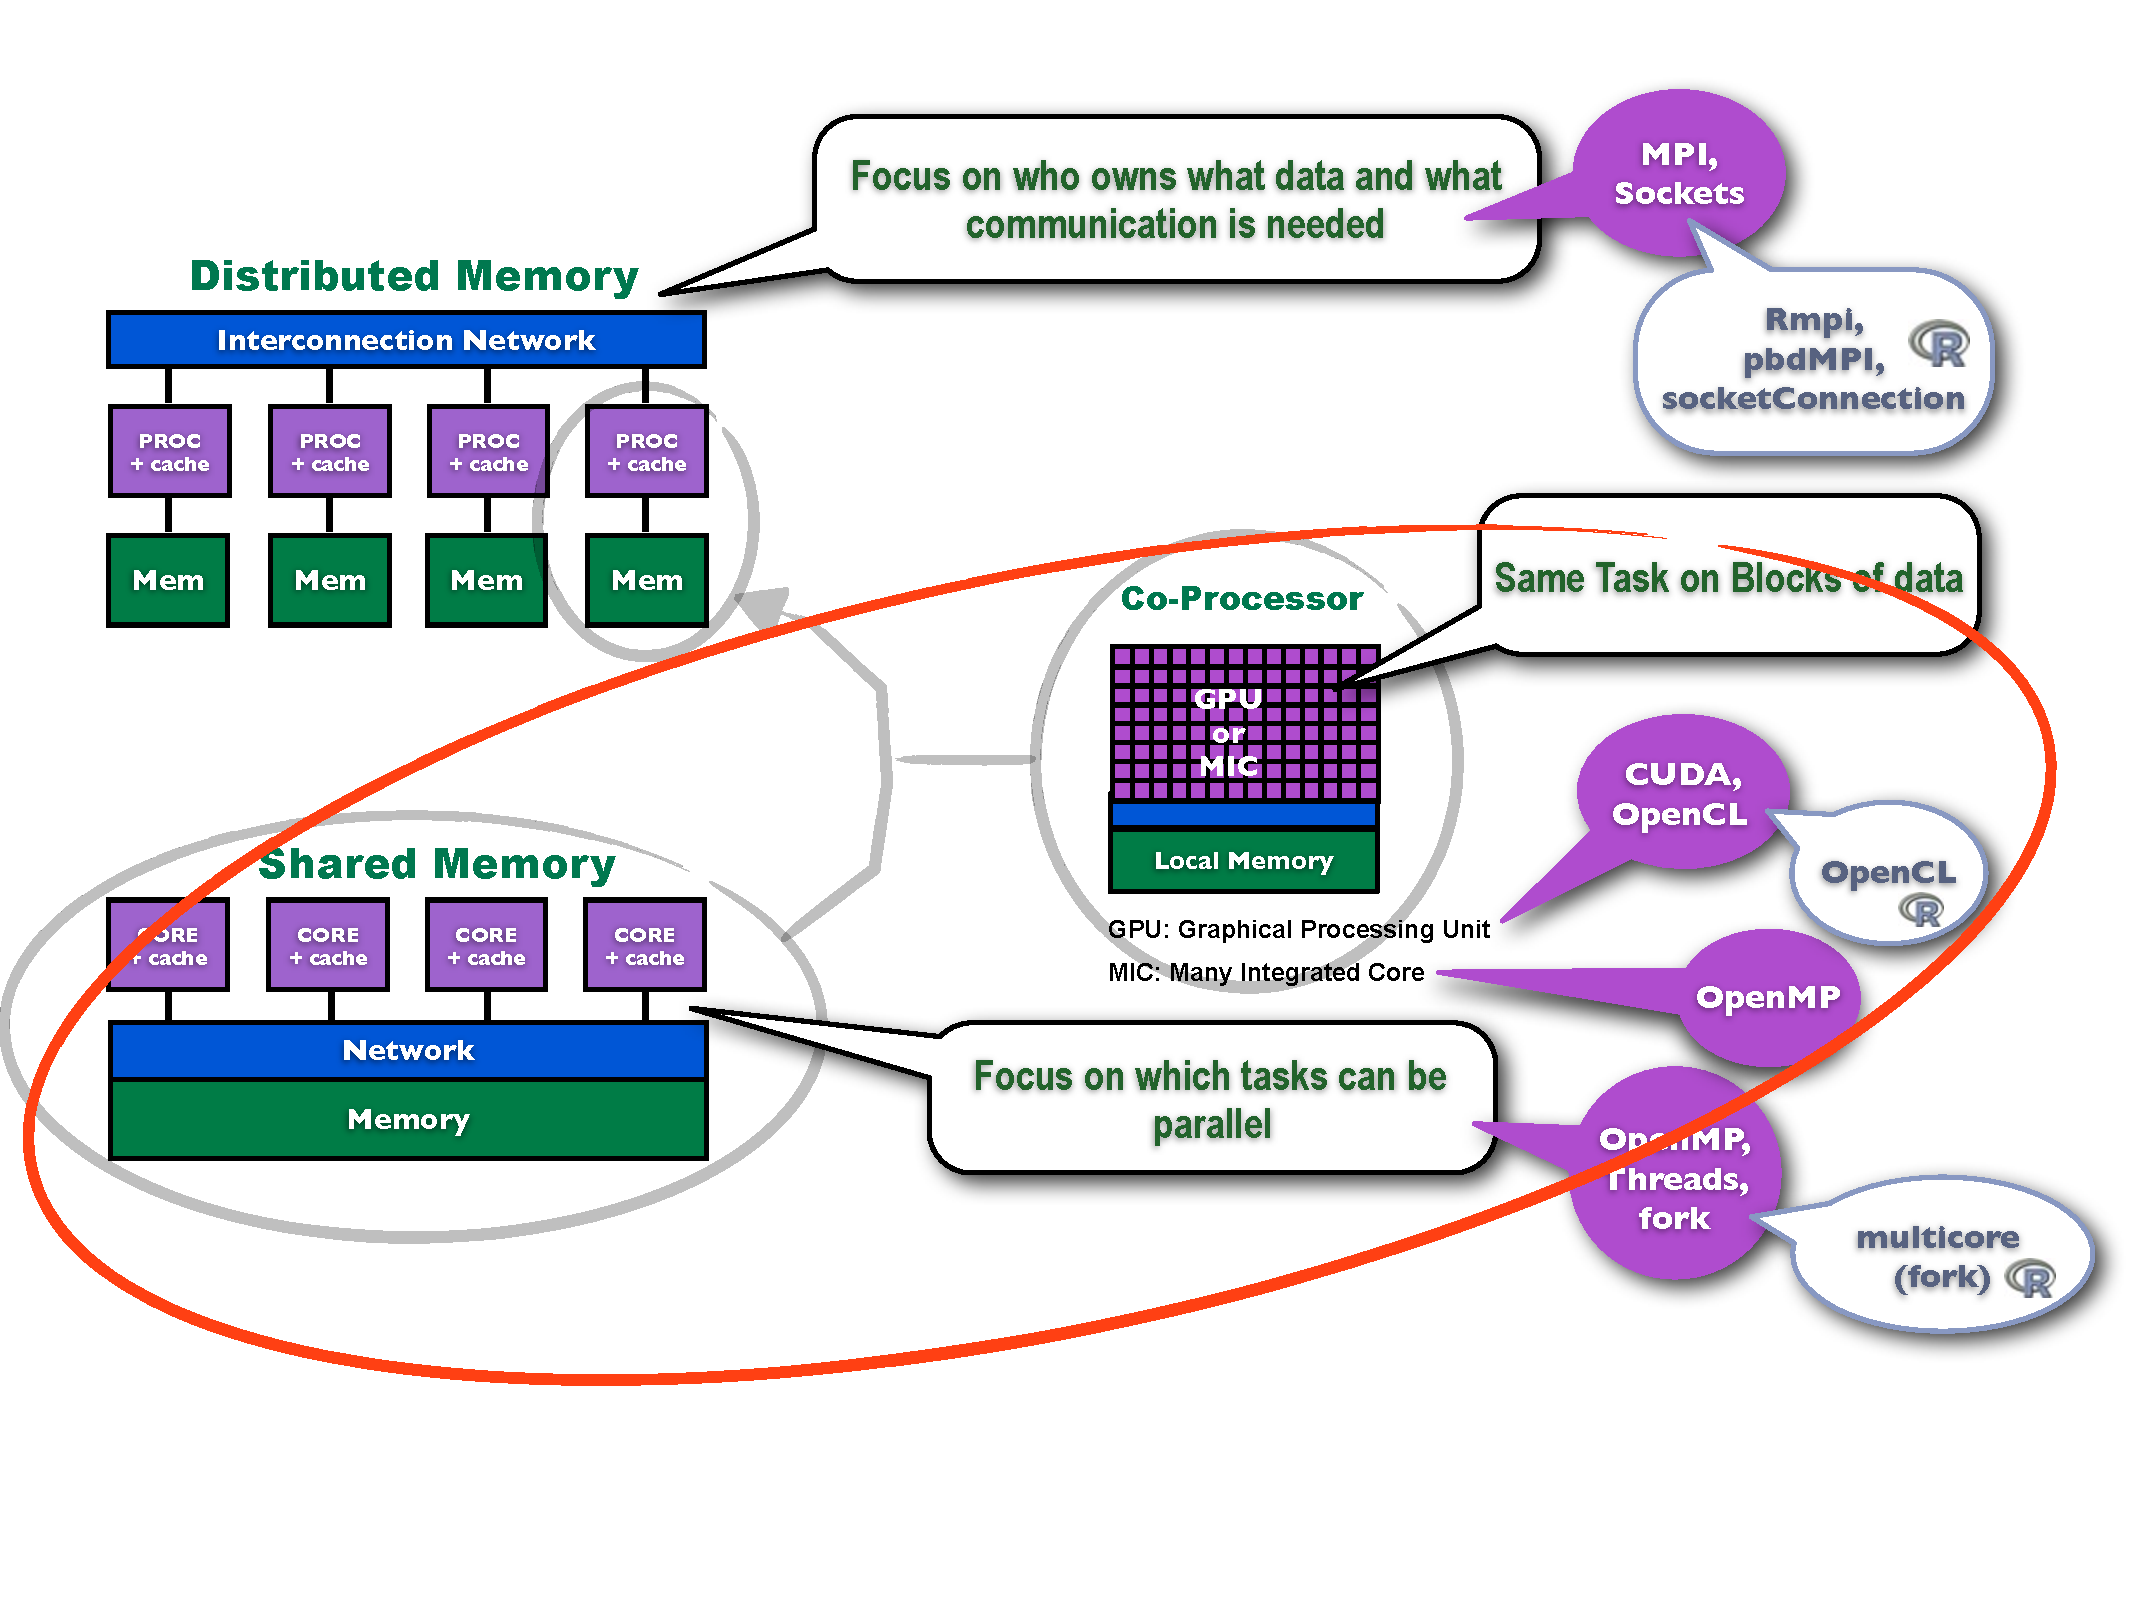
\includegraphics[width=0.95\textwidth]{../common/pics/ParallelHardware9.pdf}
\end{block}
\end{frame}

\begin{frame}
\begin{block}{Putting It All Together Challenge}
    
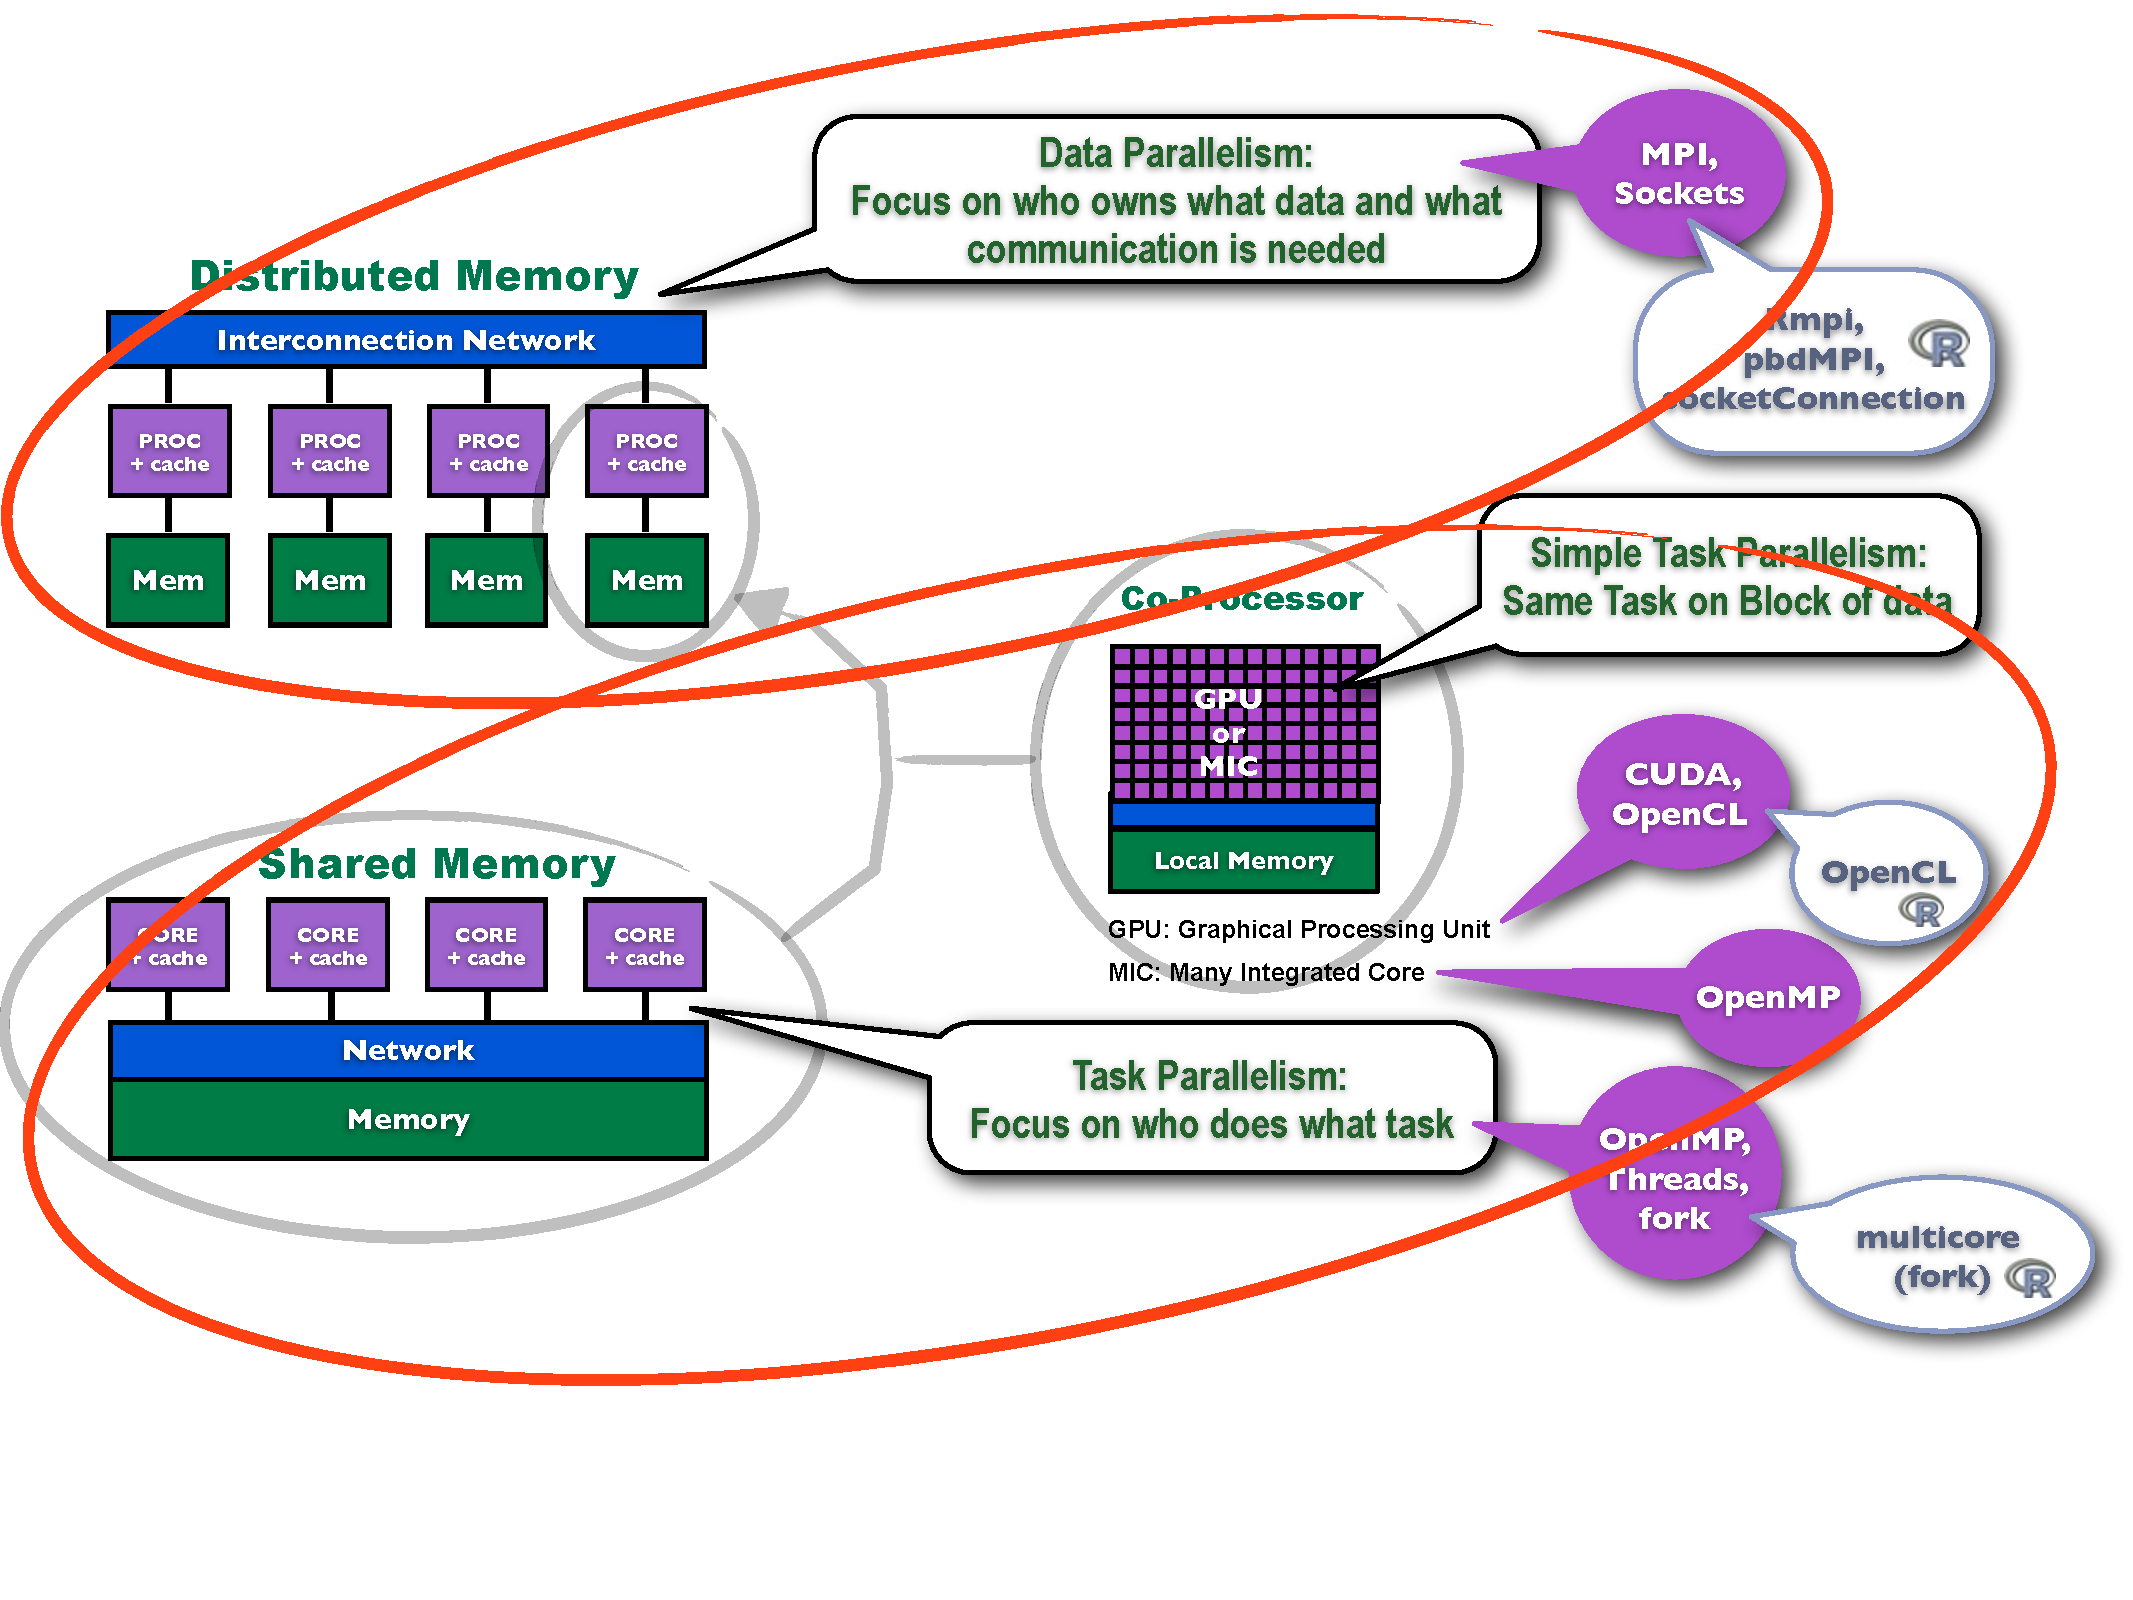
\includegraphics[width=0.95\textwidth]{../common/pics/ParallelHardware10.pdf}
\end{block}
\end{frame}

\begin{frame}
\begin{block}{pbdR Focus on Data Parallelism}
    
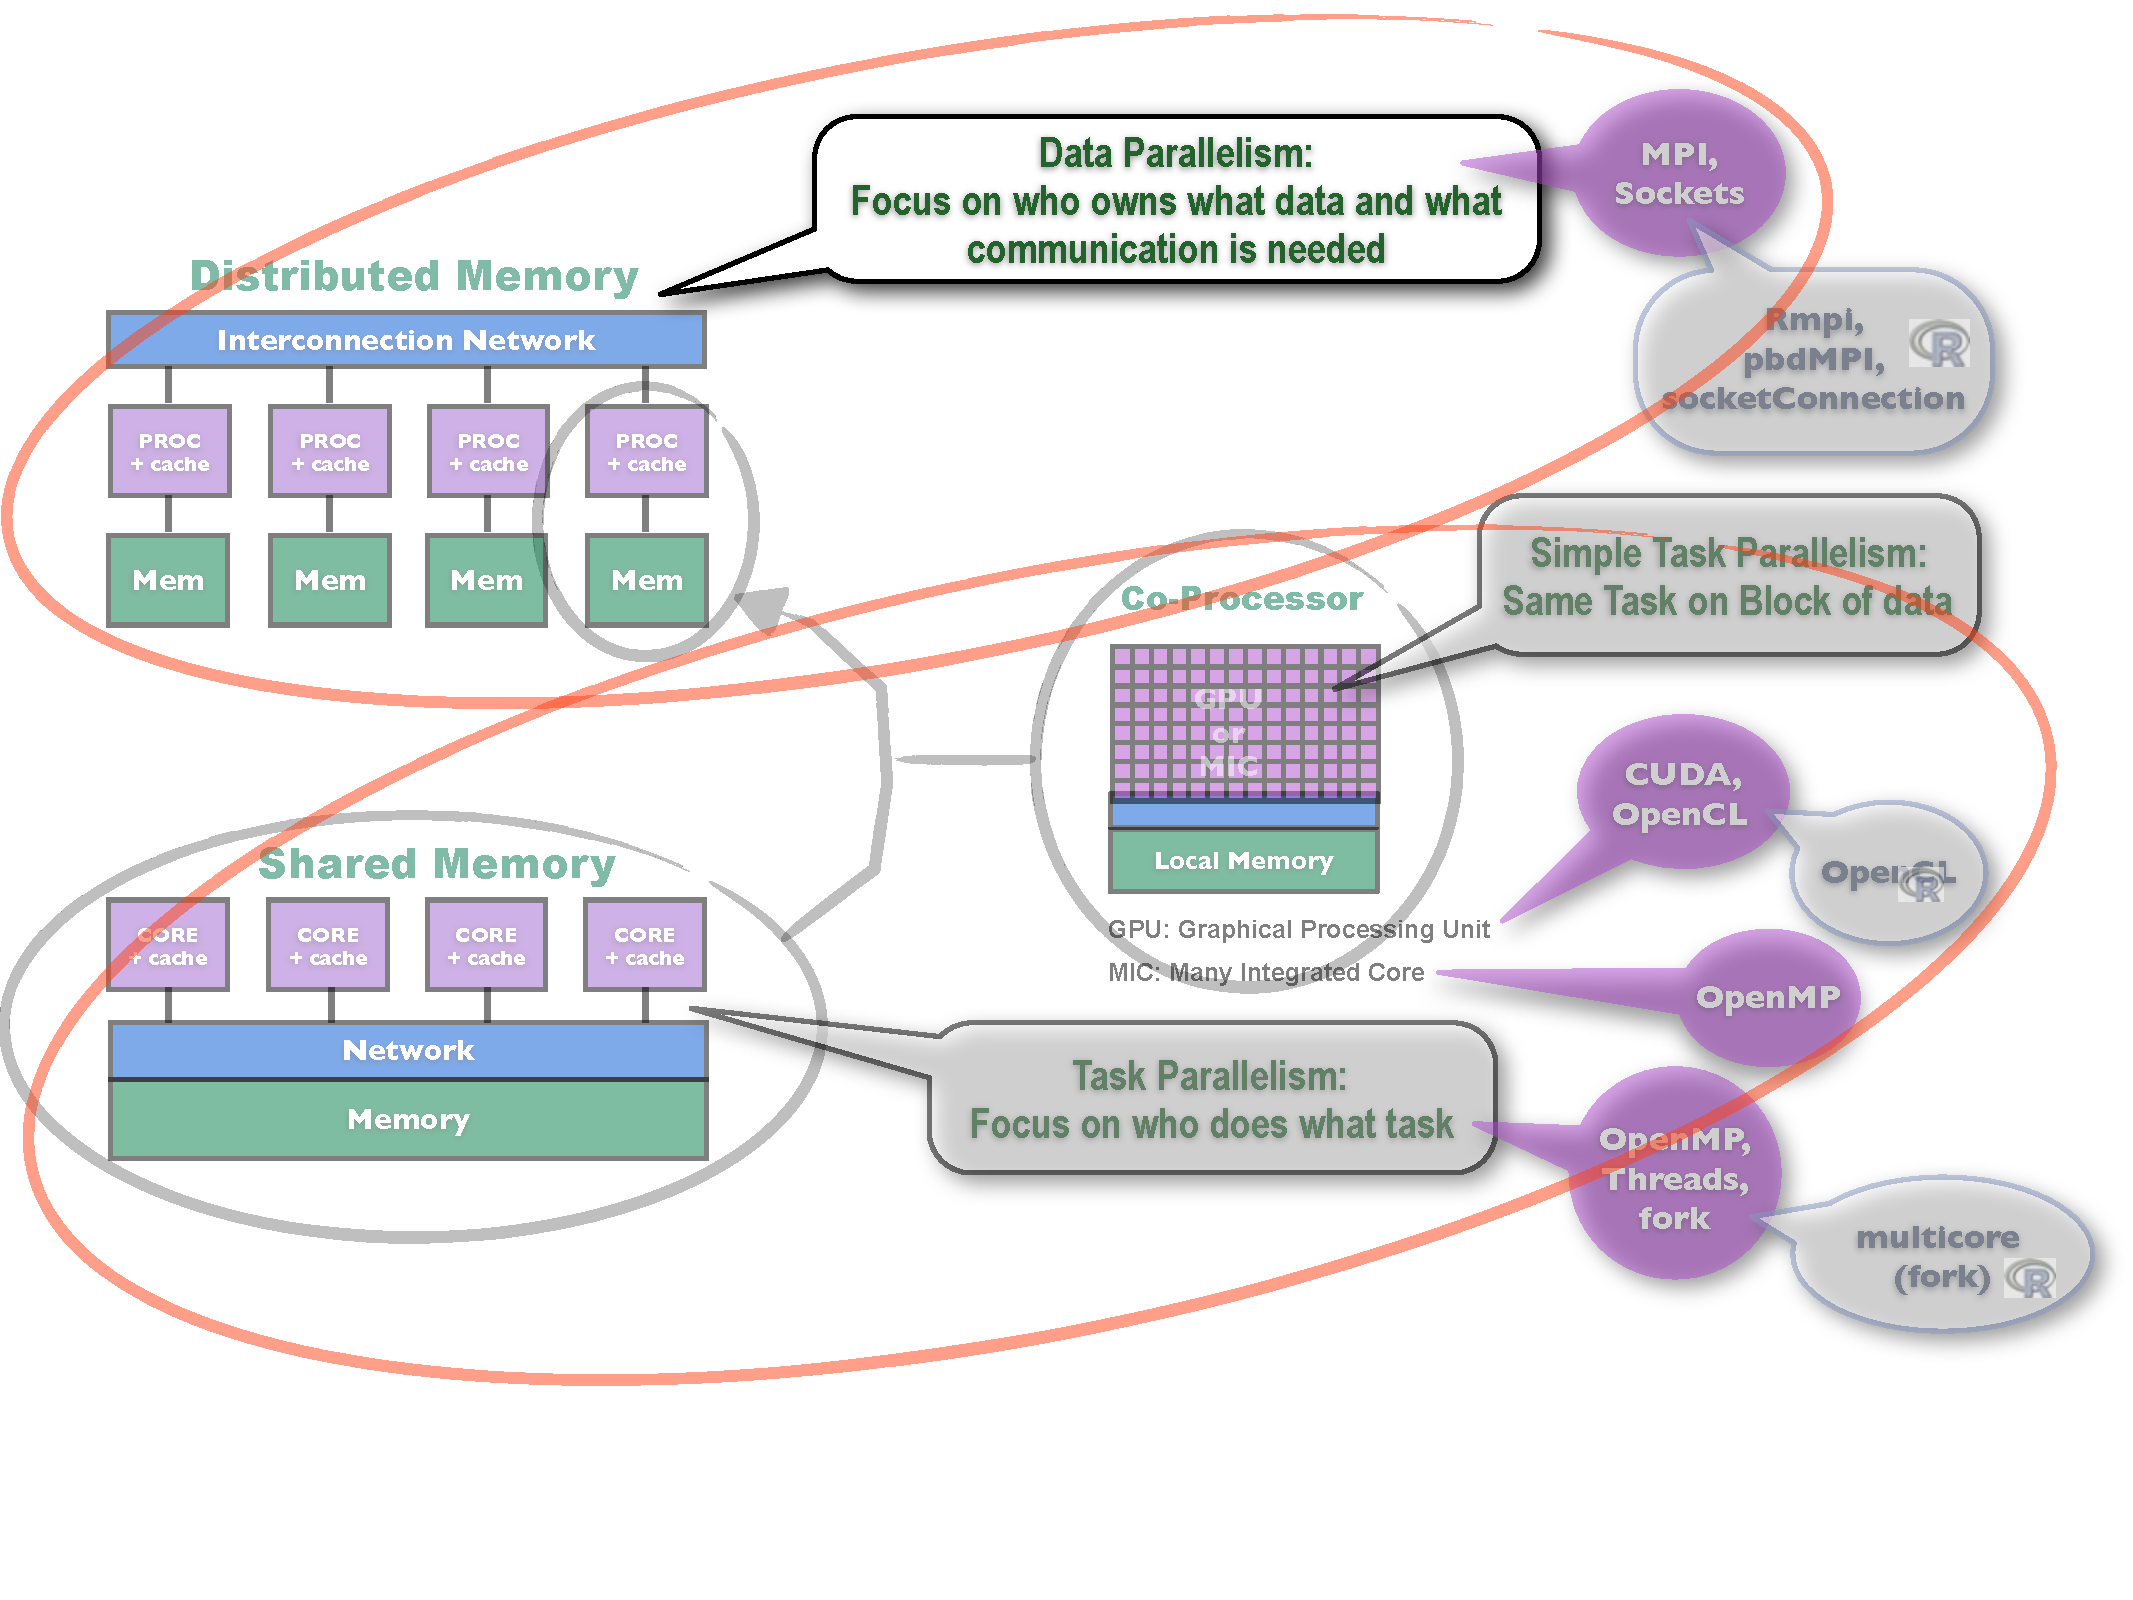
\includegraphics[width=0.95\textwidth]{../common/pics/ParallelHardware11.pdf}
\end{block}
\end{frame}
\subsection{pbdR Connects R to HPC Libraries}

\begin{frame}
\begin{block}{HPC Libraries}
    
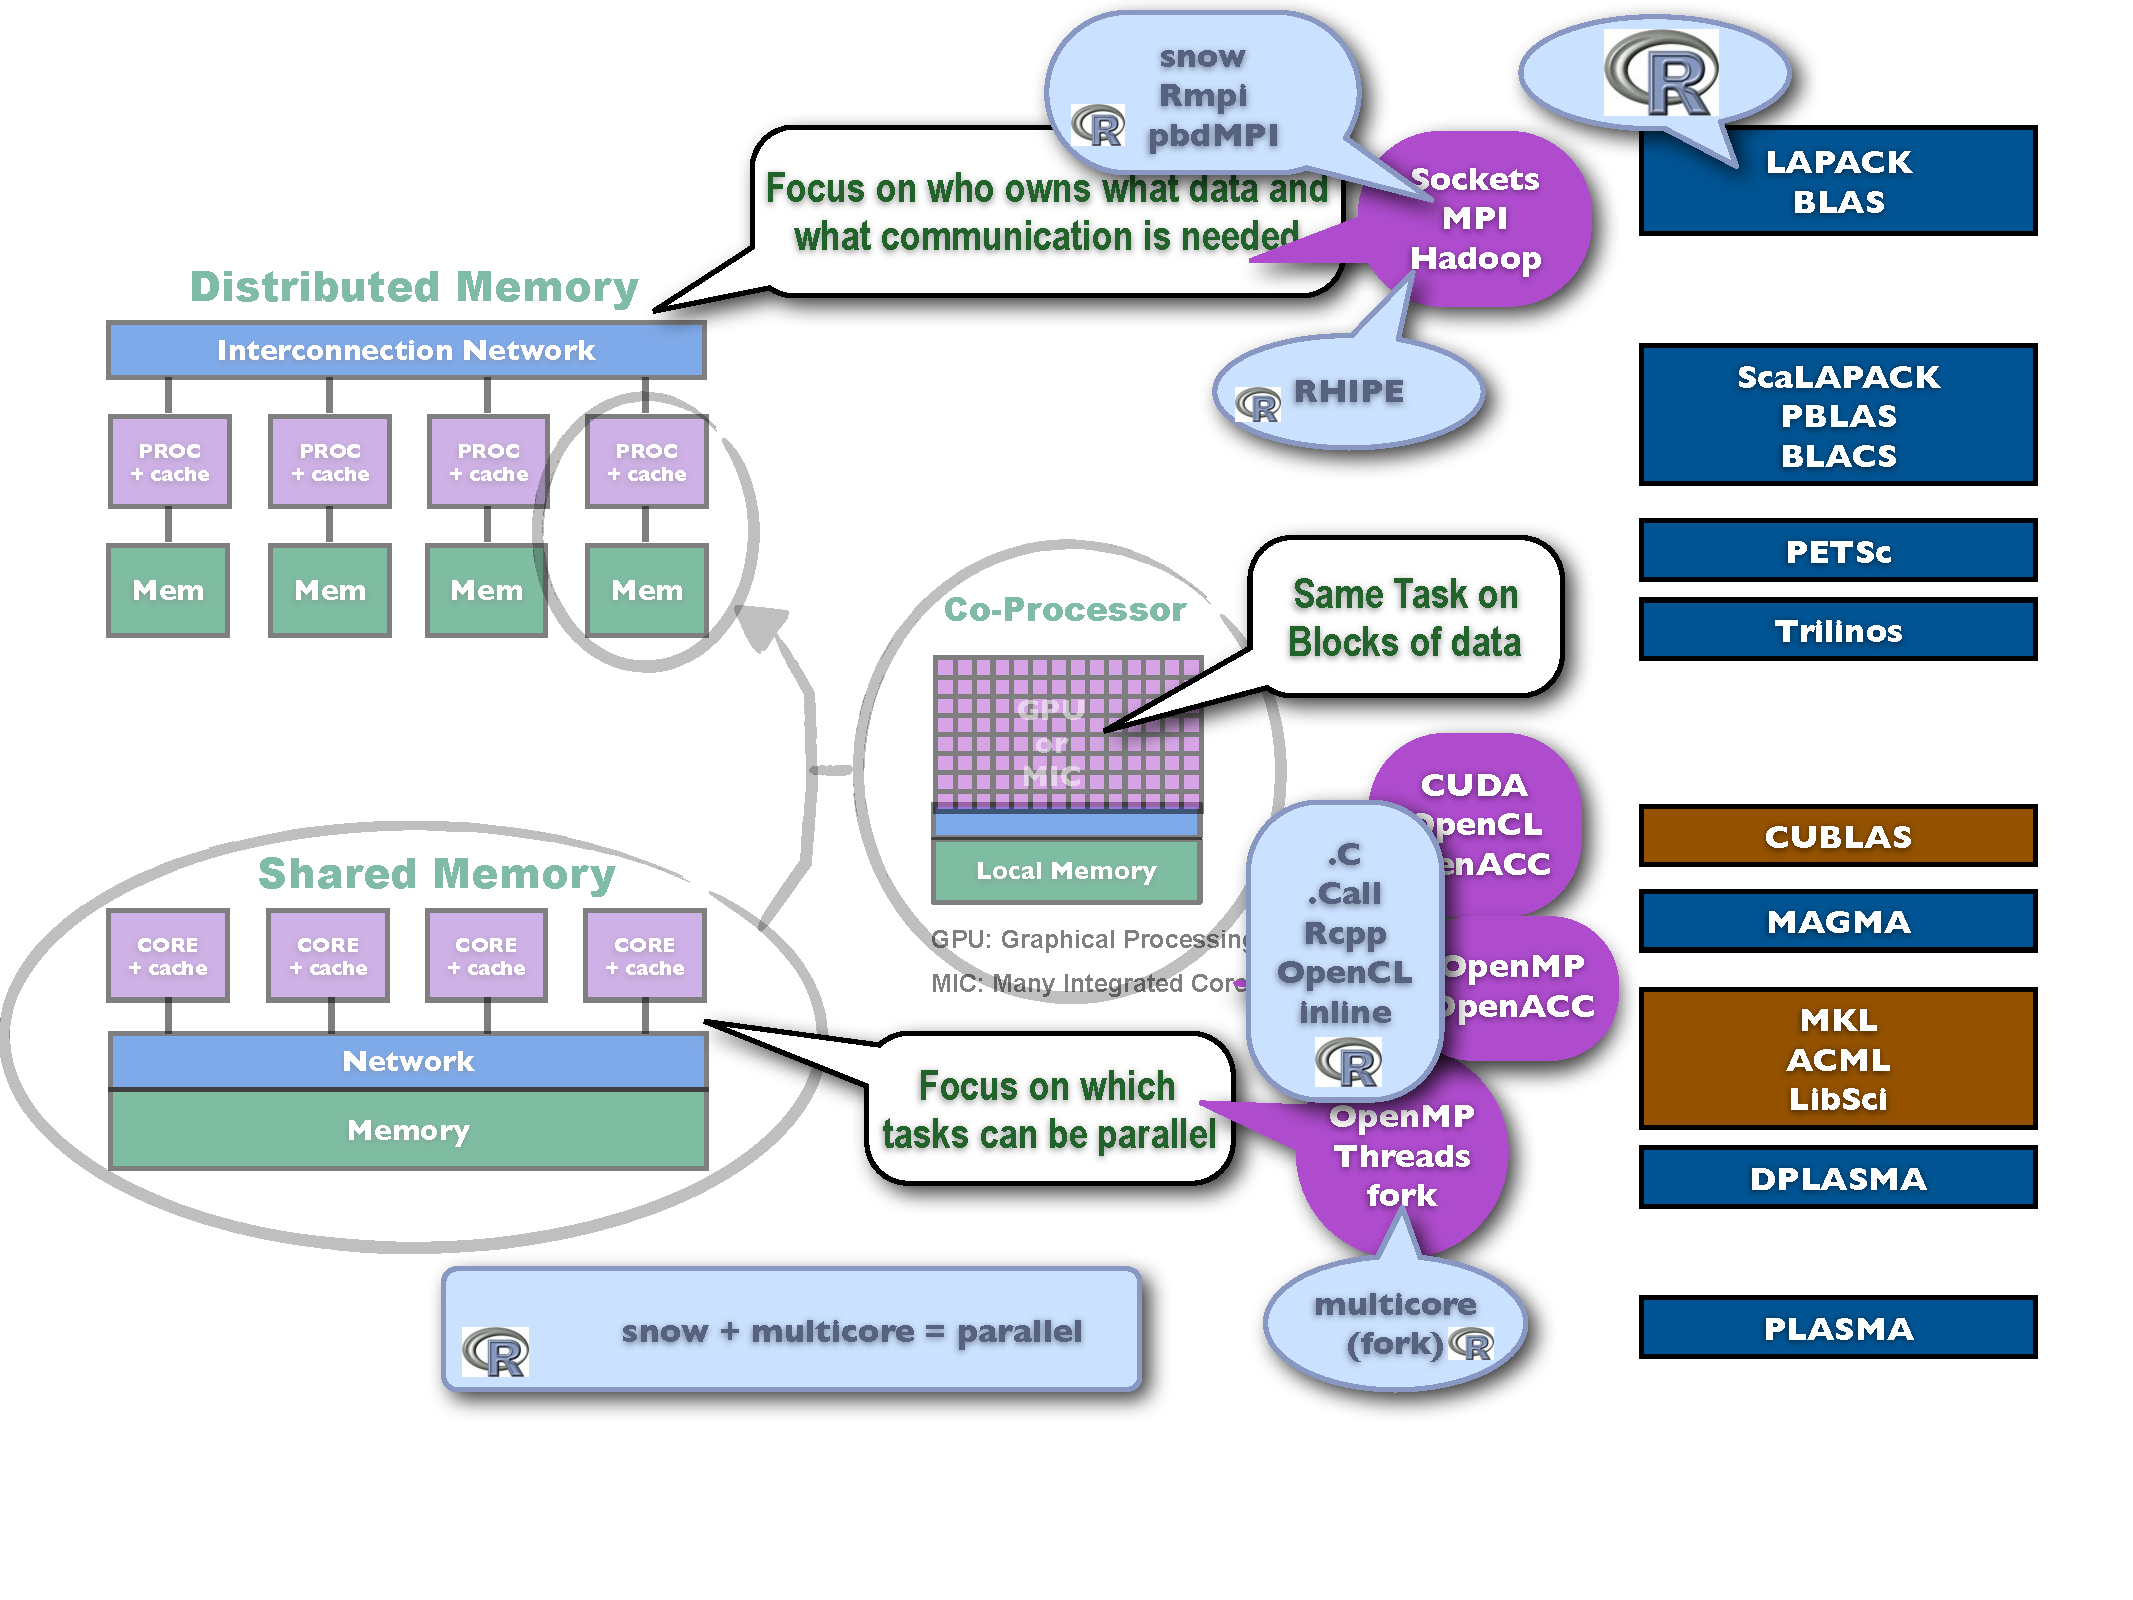
\includegraphics[width=0.95\textwidth]
{../common/pics/hardware/ParallelHardware11.pdf}
\end{block}
\end{frame}

\begin{frame}
\begin{block}{R Interfaces to Scalable HPC Libraries}
    
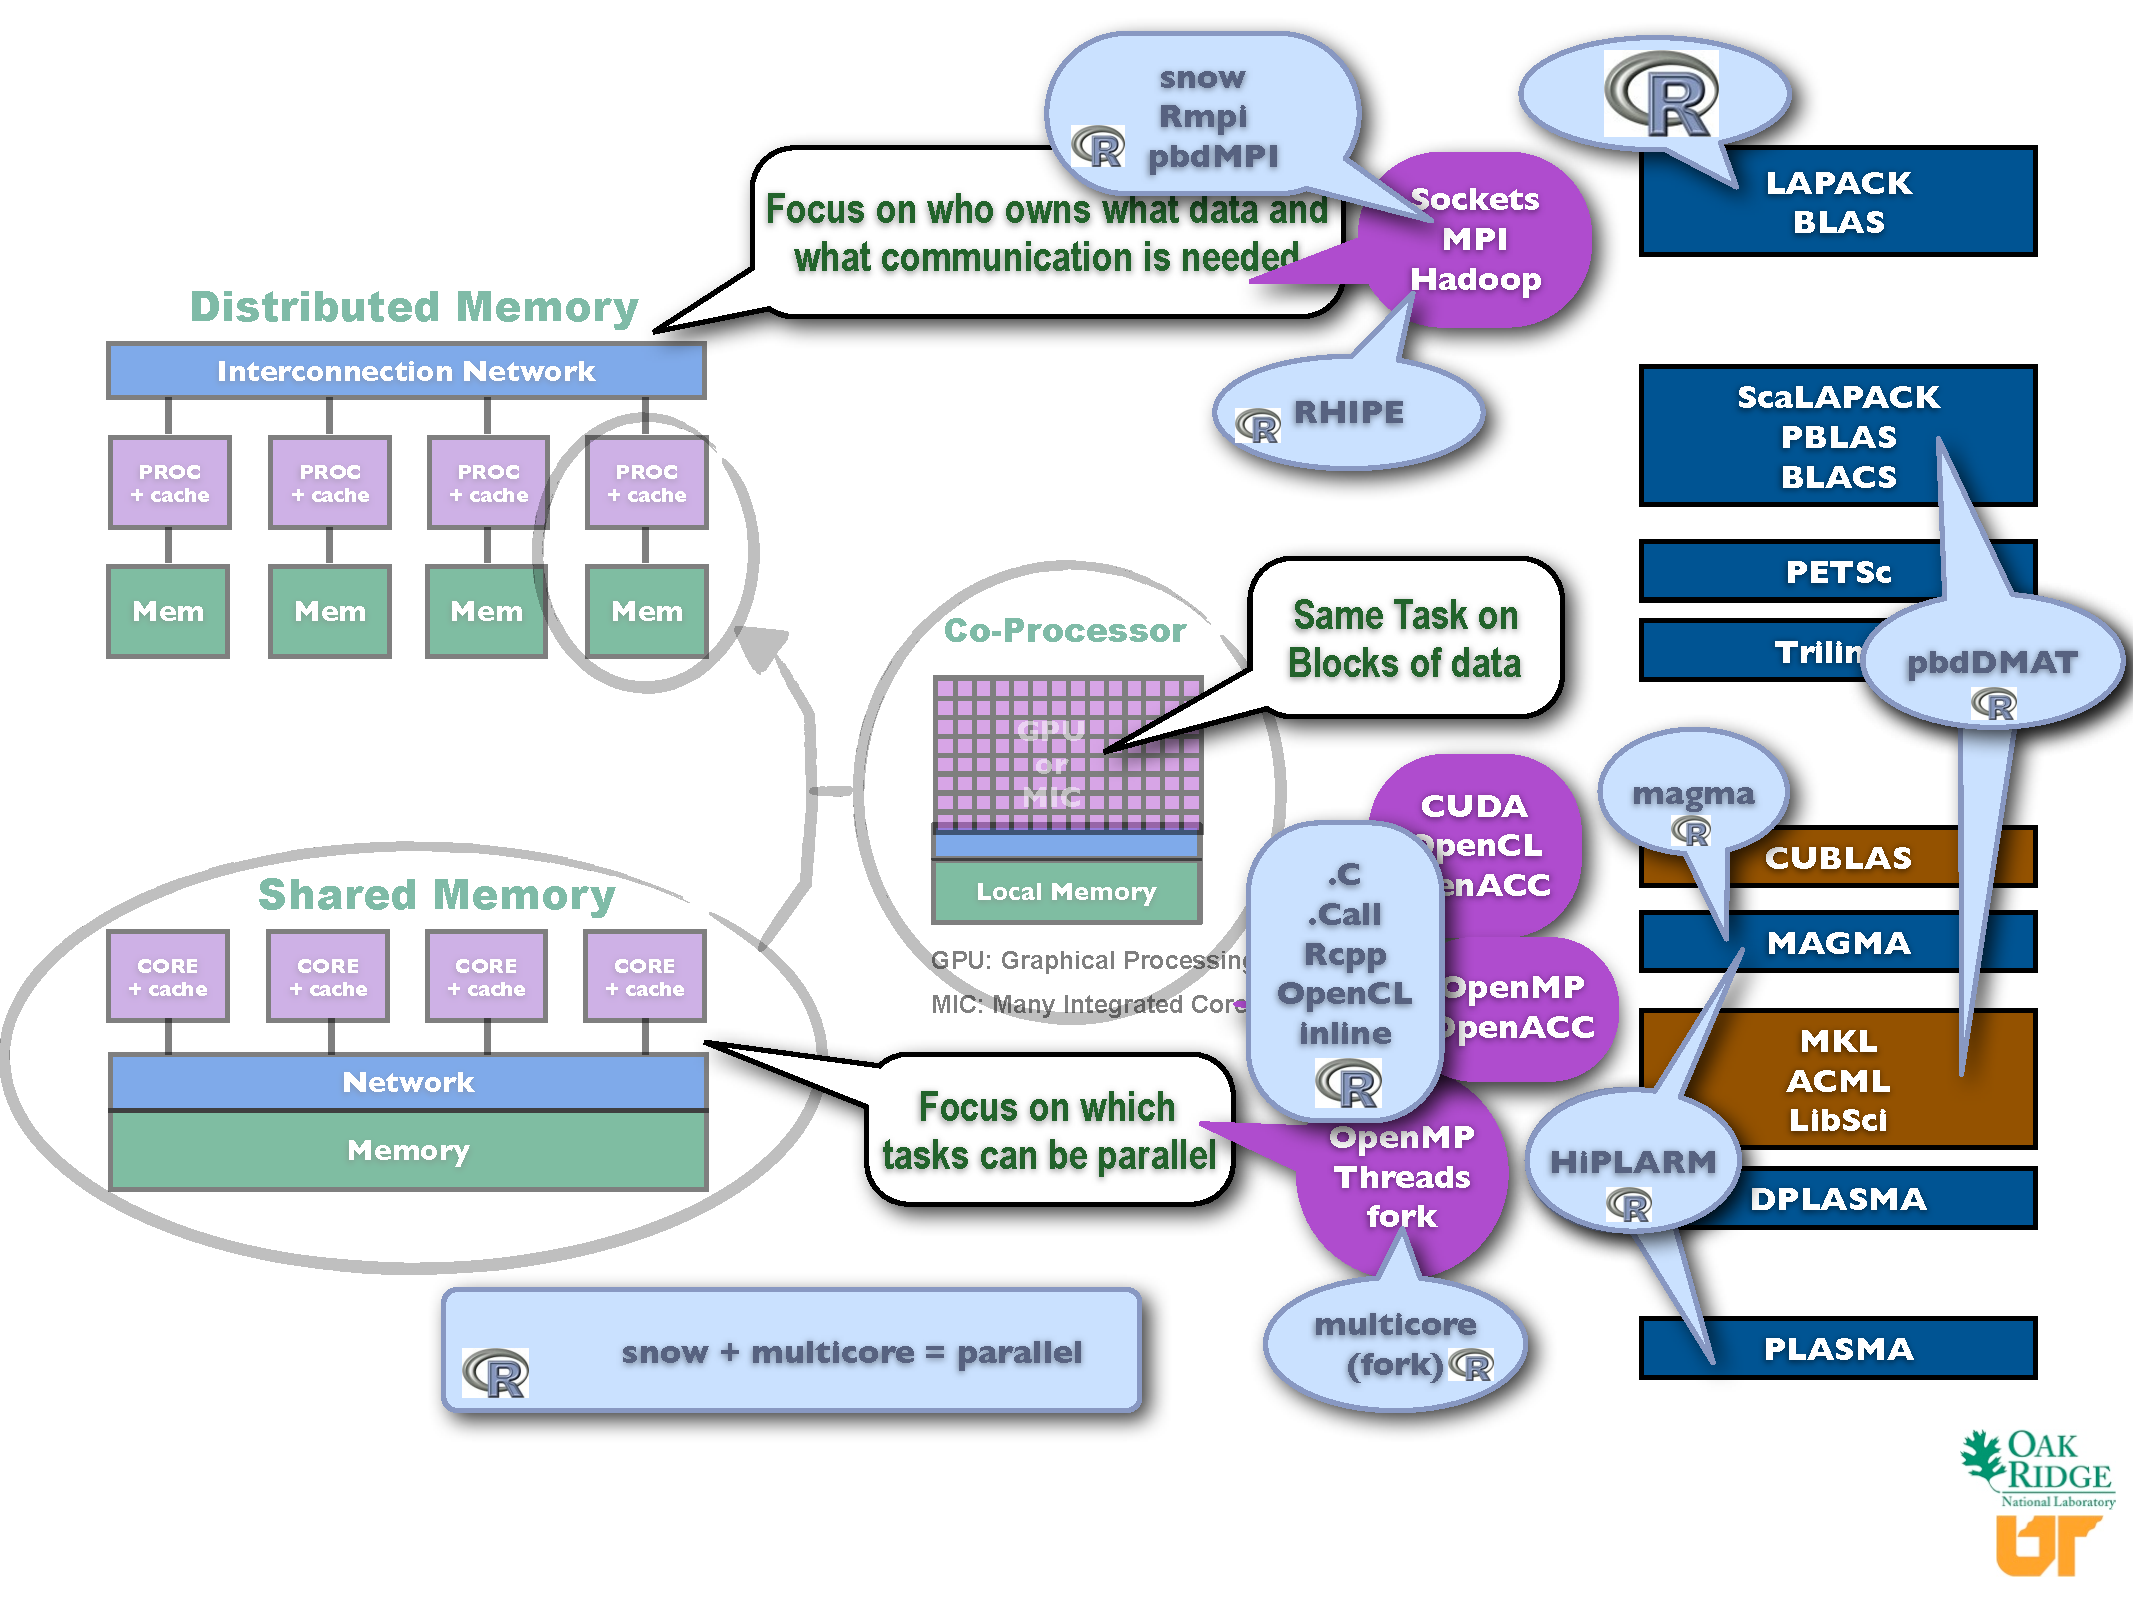
\includegraphics[width=0.95\textwidth]
{../common/pics/hardware/ParallelHardware12.pdf}
\end{block}
\end{frame}

\begin{frame}
  \begin{block}{pbdR Interfaces to Scalable HPC Libraries}
    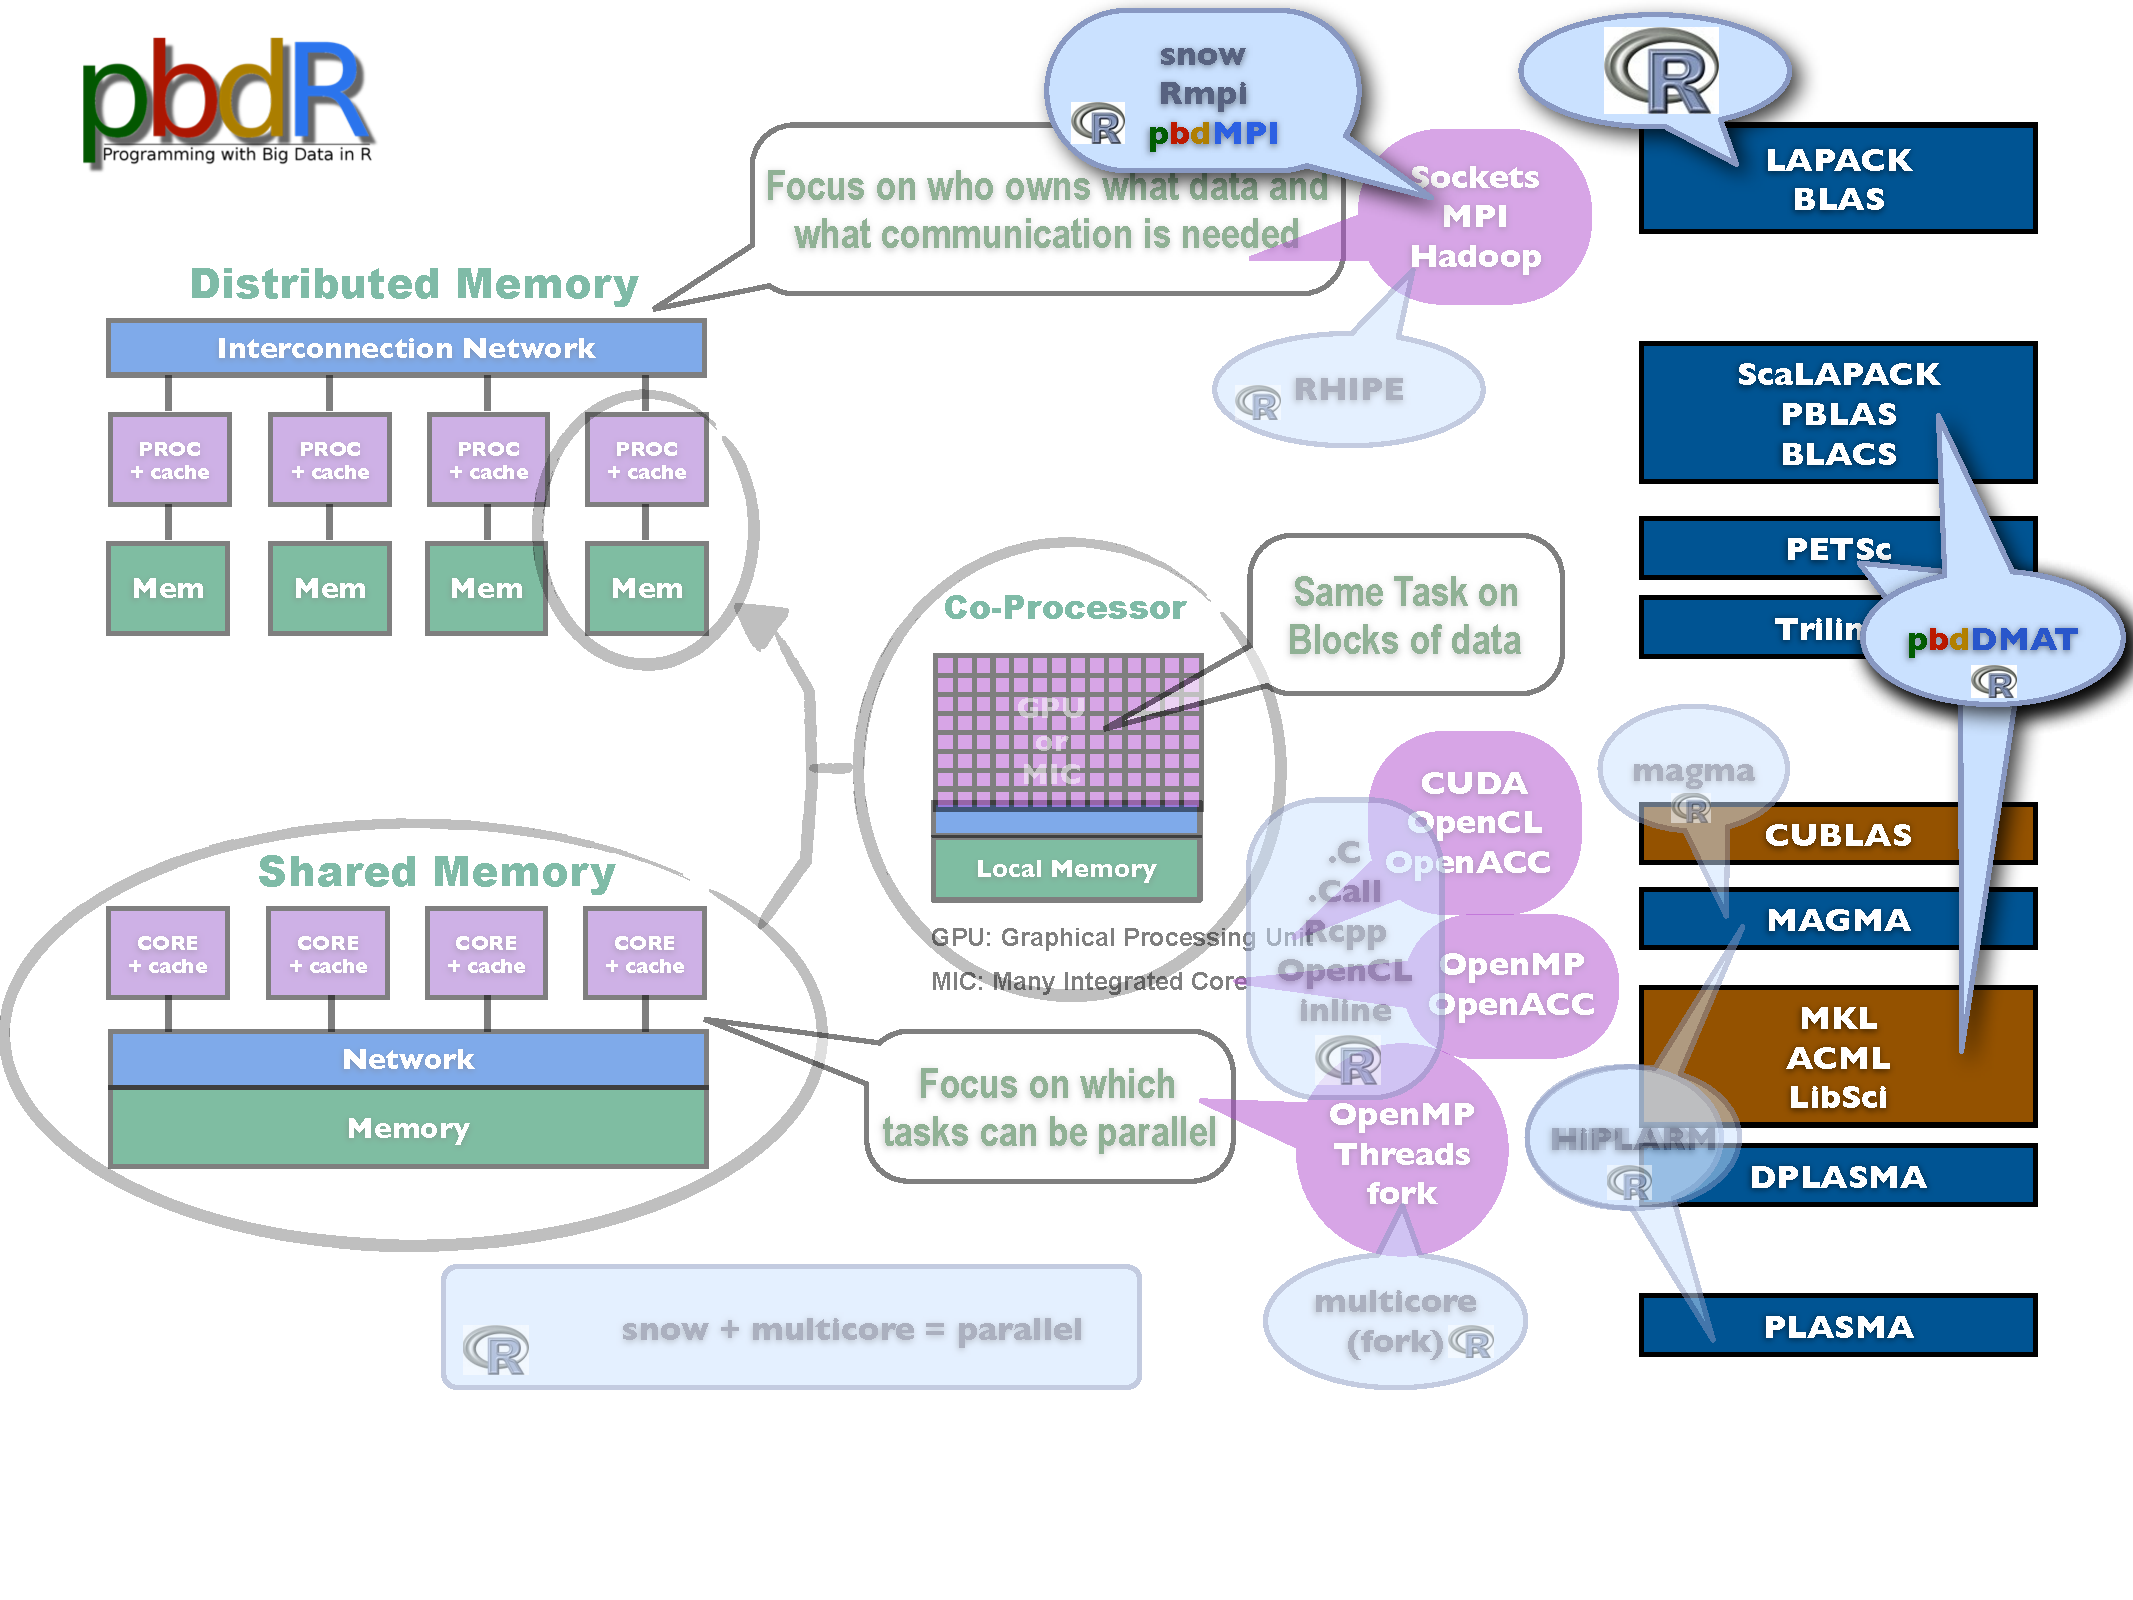
\includegraphics[width=0.95\textwidth]{../common/pics/hardware/ParallelHardware13.pdf}
  \end{block}
\end{frame}


\begin{frame}
  \begin{block}{Building R Infrastructure for Supercomputers}
    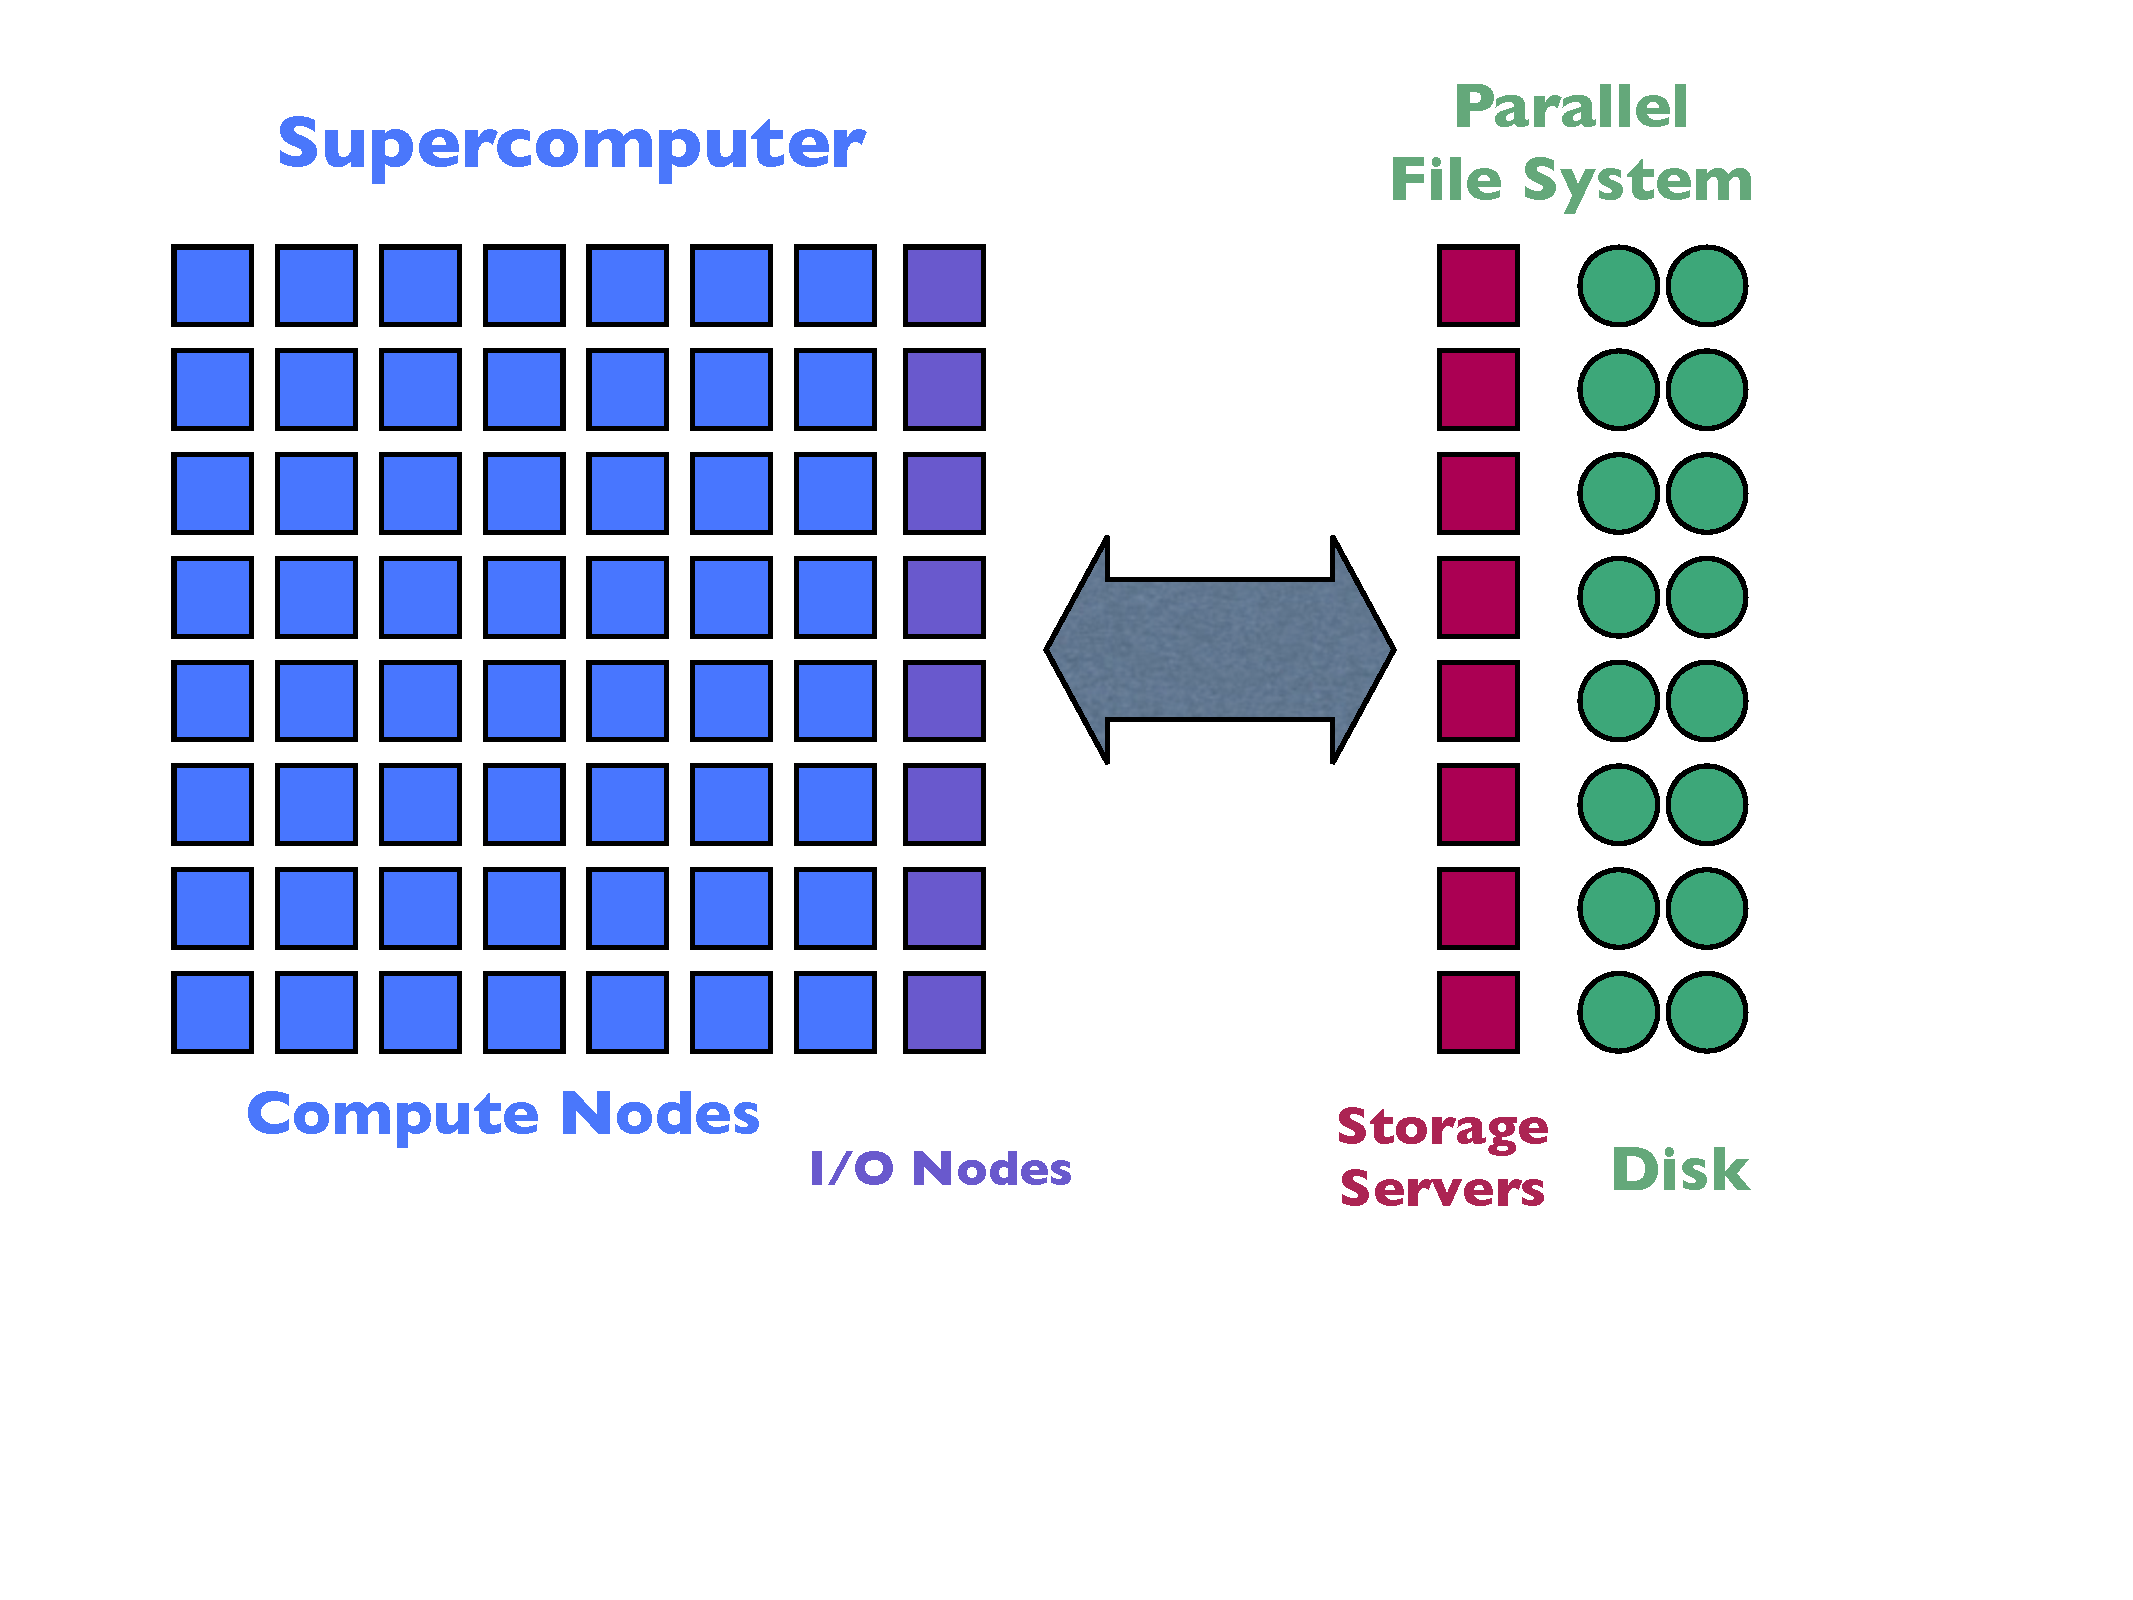
\includegraphics[width=0.95\textwidth]{../common/pics/hardware/SupercomputerFileSystem.pdf}
  \end{block}
\end{frame}


